\documentclass[11pt,leqno]{article}
\usepackage{comment}
%auto-ignore
%!TEX root = webs.tex
%this ensures the arxiv doesn't try to start TeXing here.

\usepackage{amsmath,amssymb,amsfonts,amsthm}
\usepackage{ifpdf}

\usepackage{comment}

\usepackage[all]{xy}
\SelectTips{cm}{}
% This may speed up compilation of complex documents with many xymatrices.
%\CompileMatrices

\usepackage[section]{placeins}
\usepackage{leftidx}
\usepackage{stmaryrd} % additional math symbols, e.g. \mapsfrom
%\usepackage{libertine}
%\usepackage[T1]{fontenc}
\usepackage{microtype}

% ----------------------------------------------------------------
\vfuzz5pt % Don't report over-full v-boxes if over-edge is small
\hfuzz5pt % Don't report over-full h-boxes if over-edge is small
% ----------------------------------------------------------------

% don't warn about PDF 1.5 (default was 1.4); dangerous?
\pdfminorversion=5

% diagrams -------------------------------------------------------
% figures ---------------------------------------------------------
\newcommand{\pathtotrunk}{./}
\newcommand{\pathtodiagrams}{\pathtotrunk}

\newcommand{\mathfig}[2]{\ensuremath{\hspace{-3pt}\begin{array}{c}%
  \raisebox{-2.5pt}{\includegraphics[width=#1\textwidth]{\pathtodiagrams #2}}%
\end{array}\hspace{-3pt}}}
\newcommand{\reflectmathfig}[2]{{\hspace{-3pt}\begin{array}{c}%
  \raisebox{-2.5pt}{\reflectbox{\includegraphics[width=#1\textwidth]{\pathtodiagrams #2}}}%
\end{array}\hspace{-3pt}}}
\newcommand{\rotatemathfig}[3]{{\hspace{-3pt}\begin{array}{c}%
  \raisebox{-2.5pt}{\rotatebox{#2}{\includegraphics[height=#1\textwidth]{\pathtodiagrams #3}}}%
\end{array}\hspace{-3pt}}}
\newcommand{\placefig}[2]{\includegraphics[width=#1\linewidth]{\pathtodiagrams #2}}

\newcommand{\arxiv}[1]{\href{http://arxiv.org/abs/#1}{\tt arXiv:\nolinkurl{#1}}}
\newcommand{\doi}[1]{\href{http://dx.doi.org/#1}{{\tt DOI:#1}}}
\newcommand{\euclid}[1]{\href{http://projecteuclid.org/euclid.cmp/#1}{{\tt #1}}}
\newcommand{\mathscinet}[1]{\href{http://www.ams.org/mathscinet-getitem?mr=#1}{\tt #1}}
\newcommand{\googlebooks}[1]{(preview at \href{http://books.google.com/books?id=#1}{google books})}


% THEOREMS -------------------------------------------------------
\theoremstyle{plain}
%\newtheorem*{fact}{Fact}
\newtheorem{prop}{Proposition}[subsection]
\makeatletter
\@addtoreset{prop}{section}
\makeatother
\newtheorem{conj}[prop]{Conjecture}
\newtheorem{thm}[prop]{Theorem}
\newtheorem{lem}[prop]{Lemma}
\newtheorem*{lem*}{Lemma}
\newtheorem{cor}[prop]{Corollary}
\newtheorem*{cor*}{Corollary}
\newtheorem*{exc}{Exercise}
\newtheorem{defn}[prop]{Definition}         % numbered definition
\newtheorem*{defn*}{Definition}             % unnumbered definition
\newtheorem{question}{Question}
\newtheorem{property}[prop]{Property}
\newenvironment{rem}{\vspace{0.3cm}\noindent\textsl{Remark.}}{}  % perhaps looks better than rem above?
\newenvironment{example}{\vspace{0.3cm}\noindent\textbf{Example.}}{}  % perhaps looks better than rem above?
\newtheorem{rem*}[prop]{Remark}
\numberwithin{equation}{section}
%% example, claim and remark are defined in article_preamble.tex, for compatibility with beamer and PNAS


% Marginal notes in draft mode -----------------------------------
\newcounter{comment}
\newcommand{\noop}[1]{}
\newcommand{\todo}[1]{\textbf{\color[rgb]{.8,.2,.5}\small TODO: #1}}

% \mathrlap -- a horizontal \smash--------------------------------
% For comparison, the existing overlap macros:
% \def\llap#1{\hbox to 0pt{\hss#1}}
% \def\rlap#1{\hbox to 0pt{#1\hss}}
\def\clap#1{\hbox to 0pt{\hss#1\hss}}
\def\mathllap{\mathpalette\mathllapinternal}
\def\mathrlap{\mathpalette\mathrlapinternal}
\def\mathclap{\mathpalette\mathclapinternal}
\def\mathllapinternal#1#2{%
\llap{$\mathsurround=0pt#1{#2}$}}
\def\mathrlapinternal#1#2{%
\rlap{$\mathsurround=0pt#1{#2}$}}
\def\mathclapinternal#1#2{%
\clap{$\mathsurround=0pt#1{#2}$}}

% MATH -----------------------------------------------------------
\newcommand{\id}{\boldsymbol{1}}
\renewcommand{\imath}{\mathfrak{i}}
\renewcommand{\jmath}{\mathfrak{j}}

\newcommand{\ssum}[1]{\Sigma#1}
\newcommand{\sumhat}{\overline{\sum}}
\newcommand{\sumtah}{\underline{\sum}}

\newcommand{\lmod}[1]{\leftidx{_{#1}}{\operatorname{mod}}{}}

\newcommand{\into}{\hookrightarrow}
\newcommand{\onto}{\twoheadrightarrow}
\newcommand{\iso}{\cong}
\newcommand{\quism}{\underset{\text{q.i.}}{\simeq}}
\newcommand{\htpy}{\simeq}
\newcommand{\actsOn}{\circlearrowright}
\newcommand{\xto}[1]{\xrightarrow{#1}}
\newcommand{\isoto}{\xto{\iso}}
\newcommand{\quismto}{\xrightarrow[\text{q.i.}]{\iso}}
\newcommand{\diffeoto}{\xrightarrow[\text{diffeo}]{\iso}}
\newcommand{\htpyto}{\xrightarrow[\text{htpy}]{\htpy}}

\newcommand{\restrict}[2]{#1{}_{\mid #2}{}}
\newcommand{\set}[1]{\left\{#1\right\}}
\newcommand{\setc}[2]{\setcl{#1}{#2}}
\newcommand{\setcl}[2]{\left\{ \left. #1 \;\right| \; #2 \right\}}
\newcommand{\setcr}[2]{\left\{ #1 \;\left| \; #2 \right\}\right.}

\newcommand{\floor}[1]{\left\lfloor#1\right\rfloor}
\newcommand{\norm}[1]{\left|\left|#1\right|\right|}
\newcommand{\abs}[1]{\left|#1\right|}

\newcommand{\qi}[2][q]{\left[#2\right]_{#1}}
\newcommand{\qBinomial}[3][q]{\genfrac{[}{]}{0pt}{}{#2}{#3}_{#1}}
\newcommand{\qPoch}[3]{\left(#1;#2\right)_{#3}}

\newcommand{\card}[1]{\sharp{#1}}

\newcommand{\bdy}{\partial}
\newcommand{\compose}{\circ}
\newcommand{\eset}{\emptyset}

\newcommand{\directSum}{\oplus}
\newcommand{\DirectSum}{\bigoplus}
\newcommand{\tensor}{\otimes}
\newcommand{\Tensor}{\bigotimes}

\newcommand{\Homa}[3]{\Hom_{#1}\left(#2,#3\right)}
\newcommand{\Hom}{\operatorname{Hom}}
\newcommand{\End}[1]{\operatorname{End}\left(#1\right)}

% ----------------------------------------------------------------

\ifpdf
	\usepackage[pdftex,plainpages=false,hypertexnames=false,pdfpagelabels]{hyperref}
	\usepackage[pdftex]{graphicx}
\else
	\usepackage[plainpages=false,hypertexnames=false,pdfpagelabels]{hyperref}
	\usepackage{graphicx}
\fi

%must load tikz after graphicx
\usepackage{tikz}
\usetikzlibrary{shapes}
\usetikzlibrary{backgrounds}
\usetikzlibrary{decorations,decorations.pathreplacing,decorations.markings}
\usetikzlibrary{fit,calc,through}
\usetikzlibrary{external}

\tikzstyle{mid>}=[decoration={markings, mark=at position 0.5 with {\arrow{>}}}, postaction={decorate}]
\tikzstyle{mid<}=[decoration={markings, mark=at position 0.5 with {\arrow{<}}}, postaction={decorate}]
\tikzstyle{upper>}=[decoration={markings, mark=at position 0.8 with {\arrow{>}}}, postaction={decorate}]
\tikzstyle{upper<}=[decoration={markings, mark=at position 0.8 with {\arrow{<}}}, postaction={decorate}]
\tikzstyle{lower>}=[decoration={markings, mark=at position 0.2 with {\arrow{>}}}, postaction={decorate}]
\tikzstyle{lower<}=[decoration={markings, mark=at position 0.2 with {\arrow{<}}}, postaction={decorate}]

\def\Foam{{\mathcal{F}{\rm oam}}}
\newcommand{\alt}{\wedge}
\newcommand{\Alt}[2]{{\textstyle\bigwedge^{#1}_{#2}}}
\newcommand{\Usl}[1]{U\sl_{#1}}
\newcommand{\one}{1}
\def\sA{\mathcal{A}}
\def\l{\lambda}
\def\bZ{{\mathbb{Z}}}
\def\sl{{\mathfrak{sl}}}
\def\Sp{{\mathcal{S}p}}
\def\FSp{{\mathcal{FS}p}}
\def\bC{{\mathbb{C}}}
\def\g{{\mathfrak{g}}}
\def\SL{{\rm{SL}}}
\def\GL{{\rm{GL}}}
\def\gl{{\mathfrak{gl}}}
\def\dU{\dot{{\mathcal{U}}}_q}
\def\Uq{\mathcal{U}_q}
\def\Rep{\mathcal{R}ep}
\def\la{\langle}
\def\ra{\rangle}
\def\dalg{\dot{{U}}_q}

\newcommand{\ul}[1]{{\underline{#1}}}

%\newcommand{\RepSL}[1]{\mathcal{R}ep(SL_{#1})}
\newcommand{\Lad}{\mathcal{L}ad}

\usepackage{environ}
\usepackage{xargs}

\newcommandx{\NewEnvironx}[5][2,3]{%
  \expandafter\newcommandx\csname start#1\endcsname[#2][#3]{#4}%
  \NewEnviron{#1}{\csname start#1\expandafter\endcsname\BODY #5}}

\newcommand{\ladderX}{1.5}
\newcommand{\ladderY}{1.5}
\newcommand{\ladderR}{0.6}
\newcommand{\laddercoordinates}[2]{
\foreach \x in {0,...,#1} {
	\foreach \y in {0,...,#2} {
		\coordinate (l\x\y) at (\x * \ladderX, \y * \ladderY);
		\coordinate (u\x\y) at ($(l\x\y)+\ladderR*(0,\ladderY)$);
		\coordinate (d\x\y) at ($(l\x\y)+(0,\ladderY)-\ladderR*(0,\ladderY)$);
	}
}
}
\newcommand{\ladderEn}[5]{
\draw[mid>] (l#1#2) -- (d#1#2);
\draw[mid>] (d#1#2) -- ($(l#1#2)+(0,\ladderY)$) node[left] {#3};
\draw[mid>] ($(l#1#2)+(\ladderX,0)$) -- ($(u#1#2)+(\ladderX,0)$);
\draw[mid>] ($(u#1#2)+(\ladderX,0)$) -- ($(l#1#2)+(\ladderX,\ladderY)$) node[right] {#4};
\draw[mid>] (d#1#2) --node[above]{#5} ($(u#1#2)+(\ladderX,0)$);
}
\newcommand{\ladderE}[4]{\ladderEn{#1}{#2}{#3}{#4}{}}
\newcommand{\ladderFn}[5]{
\draw[mid>] (l#1#2) -- (u#1#2);
\draw[mid>] (u#1#2) -- ($(l#1#2)+(0,\ladderY)$) node[left] {#3};
\draw[mid>] ($(l#1#2)+(\ladderX,0)$) -- ($(d#1#2)+(\ladderX,0)$);
\draw[mid>] ($(d#1#2)+(\ladderX,0)$) -- ($(l#1#2)+(\ladderX,\ladderY)$) node[right] {#4};
\draw[mid>] ($(d#1#2)+(\ladderX,0)$) --node[above]{#5} (u#1#2);
}
\newcommand{\ladderF}[4]{\ladderFn{#1}{#2}{#3}{#4}{}}
\newcommand{\ladderIn}[3]{\draw[mid>] (l#1#2) -- +($#3*(0,\ladderY)$);}
\newcommand{\ladderI}[2]{\ladderIn{#1}{#2}{1}}

\NewEnvironx{ladder}[2]{%
  \begin{tikzpicture}[baseline=13*\ladderY*#2]\laddercoordinates{#1}{#2}}
{\end{tikzpicture}}

\newcommand{\fuse}[3]{\tikz[baseline=0.5cm]{
\coordinate (z1) at (0,0);
\coordinate (z2) at (1,0);
\coordinate (c) at (0.5,0.5);
\coordinate (e) at (0.5,1);
\draw[mid>] (z1) node[below] {$#1$} -- (c);
\draw[mid>] (z2) node[below] {$#2$} -- (c);
\draw[mid>] (c) -- (e) node[above] {$#3$};
}}
\newcommand{\fork}[3]{\tikz[baseline=0.5cm]{
\coordinate (z1) at (0,1);
\coordinate (z2) at (1,1);
\coordinate (c) at (0.5,0.5);
\coordinate (e) at (0.5,0);
\draw[mid<] (z1) node[above] {$#1$} -- (c);
\draw[mid<] (z2) node[above] {$#2$} -- (c);
\draw[mid<] (c) -- (e) node[below] {$#3$};
}}


% example for creating tikz environments compatible with externalize
% thanks Andrew Stacey: http://tex.stackexchange.com/a/15614/77
%\NewEnvironx{mytikz}[1][1=]{%
%  \begin{figure}[htp]
%  \centering
%  \begin{tikzpicture}[#1]}
%{\end{tikzpicture}
%  \end{figure}}

% tricky way to iterate macros over a list
\def\semicolon{;}
\def\applytolist#1{
    \expandafter\def\csname multi#1\endcsname##1{
        \def\multiack{##1}\ifx\multiack\semicolon
            \def\next{\relax}
        \else
            \csname #1\endcsname{##1}
            \def\next{\csname multi#1\endcsname}
        \fi
        \next}
    \csname multi#1\endcsname}

% \def\cA{{\cal A}} for A..Z
\def\calc#1{\expandafter\def\csname c#1\endcsname{{\mathcal #1}}}
\applytolist{calc}QWERTYUIOPLKJHGFDSAZXCVBNM;

\usepackage{color}

% idea from tex-overflow
\usepackage{xcolor}
\definecolor{dark-red}{rgb}{0.7,0.25,0.25}
\definecolor{dark-blue}{rgb}{0.15,0.15,0.55}
\definecolor{medium-blue}{rgb}{0,0,0.65}
\hypersetup{
    colorlinks, linkcolor={dark-red},
    citecolor={dark-blue}, urlcolor={medium-blue}
}


% margin stuff
\setlength{\textwidth}{6.5in}
\setlength{\oddsidemargin}{0in}
\setlength{\evensidemargin}{0in}
\setlength{\textheight}{8.5in}
\setlength{\topmargin}{-.25in}



%\tikzexternalize[prefix=diagrams/externalized/]


\title{Webs and skew Howe duality}
\author{Sabin~Cautis, Joel~Kamnitzer and Scott~Morrison}

\begin{document}

\makeatletter
\@addtoreset{equation}{section}
\gdef\theequation{\thesection.\arabic{equation}}
\makeatother

\maketitle

\begin{abstract}
\end{abstract}

\hypersetup{
    colorlinks, linkcolor={black},
    citecolor={dark-blue}, urlcolor={medium-blue}
}

\tableofcontents

\hypersetup{
    colorlinks, linkcolor={dark-red},
    citecolor={dark-blue}, urlcolor={medium-blue}
}

\newcommand{\alt}{\wedge}

\newcommand{\Alt}{\bigwedge}

\newcommand{\Usl}[1]{U\sl_{#1}}

\newcommand{\one}{1}

\def\bZ{{\mathbb{Z}}}
\def\sl{{\mathfrak{sl}}}
\def\Sp{{\mathcal{S}p}}
\def\FSp{{\mathcal{FS}p}}
\def\bC{{\mathbb{C}}}
\def\g{{\mathfrak{g}}}
\def\SL{{\rm{SL}}}
\def\GL{{\rm{GL}}}
\def\gl{{\mathfrak{gl}}}
\def\dU{\dot{{\mathcal{U}}}_q}
\def\Uq{\mathcal{U}_q}
\def\Rep{\mathcal{R}ep}
\def\la{\langle}
\def\ra{\rangle}
% \newcommand{\gl}[1]{\mathfrak{gl}_{#1}}
%\newcommand{\Ugl}[1]{U\gl{#1}}

\newcommand{\ul}[1]{{\underline{#1}}}

%\newcommand{\RepSL}[1]{\mathcal{R}ep(SL_{#1})}
\newcommand{\Lad}{\mathcal{L}ad}

\newcommand{\ladderX}{1.5}
\newcommand{\ladderY}{1.5}
\newcommand{\ladderR}{0.6}
\newcommand{\laddercoordinates}[2]{
\foreach \x in {0,...,#1} {
	\foreach \y in {0,...,#2} {
		\coordinate (l\x\y) at (\x * \ladderX, \y * \ladderY);
		\coordinate (u\x\y) at ($(l\x\y)+\ladderR*(0,\ladderY)$);
		\coordinate (d\x\y) at ($(l\x\y)+(0,\ladderY)-\ladderR*(0,\ladderY)$);
	}
}
}
\newcommand{\ladderEn}[5]{
\draw[mid>] (l#1#2) -- (d#1#2);
\draw[mid>] (d#1#2) -- ($(l#1#2)+(0,\ladderY)$) node[left] {#3};
\draw[mid>] ($(l#1#2)+(\ladderX,0)$) -- ($(u#1#2)+(\ladderX,0)$);
\draw[mid>] ($(u#1#2)+(\ladderX,0)$) -- ($(l#1#2)+(\ladderX,\ladderY)$) node[right] {#4};
\draw[mid>] (d#1#2) --node[above]{#5} ($(u#1#2)+(\ladderX,0)$);
}
\newcommand{\ladderE}[4]{\ladderEn{#1}{#2}{#3}{#4}{}}
\newcommand{\ladderFn}[5]{
\draw[mid>] (l#1#2) -- (u#1#2);
\draw[mid>] (u#1#2) -- ($(l#1#2)+(0,\ladderY)$) node[left] {#3};
\draw[mid>] ($(l#1#2)+(\ladderX,0)$) -- ($(d#1#2)+(\ladderX,0)$);
\draw[mid>] ($(d#1#2)+(\ladderX,0)$) -- ($(l#1#2)+(\ladderX,\ladderY)$) node[right] {#4};
\draw[mid>] ($(d#1#2)+(\ladderX,0)$) --node[above]{#5} (u#1#2);
}
\newcommand{\ladderF}[4]{\ladderFn{#1}{#2}{#3}{#4}{}}
\newcommand{\ladderIn}[3]{\draw[mid>] (l#1#2) -- +($#3*(0,\ladderY)$);}
\newcommand{\ladderI}[2]{\ladderIn{#1}{#2}{1}}

\NewEnvironx{ladder}[2]{%
  \begin{tikzpicture}[baseline=13*\ladderY*#2]\laddercoordinates{#1}{#2}}
{\end{tikzpicture}}


\section{Introduction}

\subsection{Generators and relations for $ \Rep(\SL_n) $}
The representation theory of $\SL_n$ is a pivotal tensor category, and it is natural to ask for a presentation by generators and relations, as a pivotal tensor category.

There are two main choices one needs to make before looking for such a presentation. First, it would be reasonable to pass to any full subcategory, whose idempotent completion recovers the entire representation theory. In particular, in this paper we look at the full subcategory (denoted $\Rep(\SL_n)$) whose objects are isomorphic to tensor products of the fundamental representations $\Alt^k \mathbb C^n$ of $\sl_n$.  Second, we need to decide which generators to use. We take the maps $\Alt^a \mathbb{C}^n \tensor \Alt^b \mathbb{C}^n \tensor \Alt^c \mathbb{C}^n \to \mathbb{C}$. (The space of such maps is one-dimensional if $a+b+c$ is a multiple of $n$, or zero-dimensional otherwise.) It is relatively easy to show that these are indeed generators, i.e. that every $\sl_n$-linear map between tensor products of fundamental representations can be written as tensor products and compositions of these maps, along with the duality pairing and copairing maps \cite[Proposition 3.5.8]{0704.1503}. The question then, is to identify the relations holding between such planar compositions.

Said another way, we have a pivotal category (the ``free spider category'' $\FSp(\SL_n) $) of trivalent webs, with oriented edges labelled by $\{1, \ldots, n-1\}$, and at each vertex the labels summing to a multiple of $n$, and a full and dominant functor $ \FSp(\SL_n) \rightarrow \Rep(\SL_n) $. The question is to identify the pivotal ideal which is the kernel of this functor.

This problem has been studied previously. For $n=2$, there are no trivalent vertices, and the category of webs is essentially just the category of embedded 1-manifolds up to isotopy. The kernel of the functor to representation theory is the ideal generated by the difference $\tikz[baseline=-2pt]{\node[draw,circle] {};} - 2$. \todo{Explain that this is Temperley-Lieb.}

For $n=3$, generators for the kernel were determined by Kuperberg \cite{MR1403861}.  The relations allow one to remove circles, bigons, and squares.  He introduced the term ``$\SL_3$ spider" for the resulting diagrammatic category.

For $n \geq 4$, generators for the kernel have been proposed, by \cite{math.QA/0310143} (for $n=4$) and by \cite{0704.1503} (generally), but without proving that their lists of relations were complete.

This paper answers the question, in particular showing that the relations of \cite{0704.1503} are complete. In fact, those relations are over complete; just the bigon collapse, $I=H$ and `square-switch' relations suffice (and in fact only one of the square-switch relations implies the others). The relevant relations are reproduced in \S\ref{sec:diagrams}.
The main theorem, stating the isomorphism between a combinatorially defined web category $\Sp(SL_n)$ (the $\SL_n $-spider) and the representation theory of $\SL_n$, appears in \S \ref{sec:theorem}.


\subsection{Skew Howe duality and webs}
The core idea of our proof is to use skew Howe duality.  In fact we give a very succinct recipe for the relations, as certain truncations of relations holding in $\gl_m$.  We now give a quick overview of the argument.

We consider the commuting actions of $ SL_n $ and $ \gl_m $ on $\Alt^\bullet(\mathbb{C}^n \tensor \mathbb{C}^m)$.  Skew Howe duality tells us that the resulting map
\begin{equation}
\dU\gl_m \rightarrow \Hom_{\SL_n}(\Alt^K(\mathbb{C}^n \tensor \mathbb{C}^m))
\end{equation}
is surjective.  Moreover, we prove that its kernel is the ideal generated by those weight space idempotents falling outside the weight support of $\Alt^\bullet(\mathbb C^n \tensor \mathbb C^m)$.  This result is proved in \S \ref{sec:fully-faithful}.  The quotient of $ \dU\gl_m $ by this ideal is denoted $\dU^n\gl_m$.

As $\SL_n$-representations, we have
\begin{equation*}
\Alt^K(\mathbb C^n \tensor \mathbb C^m)  = \alt^L(\mathbb C^n \directSum \cdots \directSum \mathbb C^n)
         = \DirectSum_{\underline{l}: \sum \underline{l} = K} \alt^{l_1} \mathbb C^n \tensor \cdots \tensor \alt^{l_m} \mathbb C^n
\end{equation*}

Thus combining the last two equations, we obtain an isomorphism,
\begin{equation*}
\dU^n(\gl_m) \rightarrow \oplus_{\ul{l}, \ul{k} : \sum \ul{l} = \sum \ul{k}} \Hom_{\SL_n}(\alt^{l_1} \mathbb C^n \tensor \cdots \tensor \alt^{l_m} \mathbb C^n, \alt^{k_1} \mathbb C^n \tensor \cdots \tensor \alt^{k_m} \mathbb C^n)
\end{equation*}

Under this map, elements of $\gl_m $ acts by particular webs, which we call ladders.  This allows us to write the generating relations of $ \dU^n(\gl_m) $ in a diagrammatic form.  By the above isomorphism, we see that these diagrammatic relations become the generating relations in the $ \SL_n $-spider.

%We denote the quotient of the category of trivalent webs by the bigon, $I=H$ and square switch relations as $\Sp(SL_n)$. We have a surjective functor to the representation theory, which we would like to show is an isomorphism. All that remains is to check that it is injective on morphisms.

%Skew Howe duality states that the commuting actions of $\SL_n$ and $\Ugl{m}$ on $\Alt^\bullet(\mathbb{C}^n \tensor \mathbb{C}^m)$ are in fact each the commutant of the other. That is, if  $f: \Alt^\bullet(\mathbb{C}^n \tensor \mathbb{C}^m) \to \Alt^\bullet(\mathbb{C}^n \tensor \mathbb{C}^m)$ is $\SL_n$-linear, then there is some element $X_f \in \Usl{m}$ whose action on  $\Alt^\bullet(\mathbb{C}^n \tensor \mathbb{C}^m)$ is exactly $f$.

%Suppose we have some element $A \in \Homa{\Sp(SL_n)}{\underline{k}}{\underline{k'}}$ which maps to zero in the representation theory. Here $\underline{k}$ and $\underline{k}$ denote two sequences of integers with signs from the set $\{1^\pm,\ldots,n-1^\pm\}$, i.e. two objects in $\Sp(SL_n)$. (The sign indicates whether the strand and that boundary point is oriented up or down.) First, we realize that by conjugating $A$ by the isomorphisms between $k^-$ and $(n-k)^+$ in $\Sp(SL_n)$, which are sent to isomorphisms in the representation theory, we may assume that all the signs are positive.

 %We would like to show that $A$ is itself zero.
 %We then choose sequences $\ul{l}$ and $\ul{l'}$ obtained from $\underline{k}$ by interposing some number of $0$s and $n$s, so $\ul{l}$ and $\ul{l'}$ have the same length $m$ and the same sum $L$ (previously, the sums of $\underline{k}$ and $\underline{k'}$ might be differed by a multiple of $n$).
 %The element $A$ is then equivalent, via the specified relations in $\Sp(SL_n)$ to a `ladder diagram' with $m$ rails and boundary given by the sequences $\ul{l}$ and $\ul{l'}$. (See Figure \ref{fig:ladder-example} for an example.)

 \begin{figure}[ht]
\begin{equation}
\begin{ladder}{2}{3}
\node[left] at (l00) {$a$};
\node[left] at (l10) {$b$};
\node[left] at (l20) {$c$};
\ladderFn{0}{0}{$a{+}s$}{$b{-}s$}{$s$}
\ladderEn{1}{1}{\small $b{-}s{-}t$}{$c{+}t$}{$t$}
\ladderEn{0}{2}{$a{+}s{-}r$}{\small $b{-}s{-}t{+}r$}{$r$}
\ladderI{0}{1}
\ladderI{2}{0}
\ladderI{2}{2}
\end{ladder}
\end{equation}
 \caption{An example of a ladder; this one corresponds to the word $F_1^{(r)}F_2^{(t)}E_1^{(s)} \one_{abc}$ (reading bottom to top, right to left) in $\dU(\gl_3)$}
 \label{fig:ladder-example}
 \end{figure}

%A complete description of ladder diagrams and this equivalence to a ladder diagram is in \S \ref{sec:ladders}.

%Now, rewriting $\Alt^L(\mathbb C^n \tensor \mathbb C^m)$ as
%\begin{align*}
%\alt^L(\mathbb C^n \tensor \mathbb C^m) & = \alt^L(\mathbb C^n \directSum \cdots \directSum \mathbb C^n) \\
%        & = \DirectSum_{\underline{l}: \sum \underline{l} = L} \alt^{l_1} \mathbb C^n \tensor \cdots \tensor \alt^{l_m} \mathbb C^n
%\end{align*}
%we see the objects $\underline{l}$ and $\underline{l}'$ as summands, and hence $A$ as an endomorphism of $\Alt^L(\mathbb C^n \tensor \mathbb C^m)$. Thus there is some element $X_{A} \in \dU(\gl_m)$, which acts by zero on $\Alt^L(\mathbb C^n \tensor \mathbb C^m)$. In fact, since we had shown $A$ was equivalent to a ladder diagram, we can write down an explicit element $X_A$, by interpreting each rung of the ladder as some $E^{(a)}_j$ or $F^{(a)}_j$ in $\dU(\gl_m)$.




\section{$U_q(\sl_n) $ and its representations}
\subsection{The quantum group $U_q(\sl_n) $}
We denote by $[n]_q$ the quantum integer $q^{n-1} + q^{n-3} + \dots + q^{-n+3} + q^{-n+1}$. More generally,
$$\qBinomial{n}{k} := \frac{[n]_q\dots[1]_q}{([n-k]_q \dots [1]_q)([k]_q \dots [1]_q)}.$$

$U_q(\sl_n) $ is a $ \bC(q)$-algebra with generators $ E_i, F_i, K_i $ for $ i = 1, \dots, n-1 $ and relations
\begin{align*}
K_i E_i K_i^{-1} = q^2 E_i, K_i F_i K_i^{-1} = q^{-2}F_i, ...
\end{align*}
\todo{We should either fill in our leave our these relations.  I mainly put this in because I wanted to write down the coproduct.}


It is a Hopf algebra with the coproduct given by
\begin{align*}
\Delta(E_i) = E_i \otimes K_i + 1 \otimes E_i, \ \ \Delta(F_i) = F_i \otimes 1 + K_i^{-1} \otimes F_i, \ \ \Delta(K_i) = K_i \otimes K_i 
\end{align*}

\subsection{Representations of $U_q(\sl_n) $}

$U_q(\sl_n) $ has a standard representation $ \bC_q^n := \bC(q)^n $.  We use $ x_1, \dots, x_n $ for the usual basis of $ \bC_q^n $.  We define the quantum exterior algebra $\Alt^\bullet_q(\bC_q^n) $ by
$$
\Alt^\bullet_q(\bC_q^n) := T \bC_q^n / \langle S^2_q ( \bC_q^n) \rangle
$$
to be the tensor algebra (over $\bC(q) $) of $ \bC_q^n $ modulo the quantum symmetric square (see \cite{BZ}).  $ \Alt^\bullet_q(\bC_q^n) $ is a graded $U_q(\sl_n)$-module algebra. We will write $ \wedge_q $ to denote the multiplication in $ \Alt^\bullet_q(\bC_q^n) $.

Note that $S^2_q \bC_q^n $ is spanned by 
$$
x_i \otimes x_j + q x_j \otimes x_i, \text{ for }  i < j , \text{ and } x_i^2, \text{ for all } i 
$$ 
Thus in $ \Alt^\bullet_q(\bC_q^n) $ we have that
$$
x_i \wedge_q x_j - q x_j \wedge_q x_i = 0 \text{ for }  i < j, \text{ and } x_i \wedge_q x_i = 0, \text{ for all }  i . 
$$

If $ S =\{k_1, \dots, k_a\} \subset \{1, \dots, n\} $, with $ k_1 > \dots > k_a $, we write $ x^S = x_{k_1} \wedge_q \cdots \wedge_q x_{k_a} \in \Alt^a_q(\bC_q^n) $. The set $ x^S $ where $ S $ ranges over $ k $ element subsets of $ \{1, \dots, n \} $ forms a basis for $ \Alt^k_q(\bC_q^n) $.
\todo{You may wonder why $ S $ is written backwards.  I did it to make some formulas work out better later.  We can change it, but I don't see any reason to.}

We will study the category $\Rep(\SL_n)$ whose objects are representation of $\Uq(\sl_n) $ isomorphic to tensor products of the fundamental representations $\Alt^k_q \bC_q^n$ of $U_q(\sl_n)$.

\subsection{Some generating morphisms}
\label{sec:generating-morphisms}
We will now define some morphisms in $ \Rep(\SL_n) $ which we will later see generates the morphisms in this category.

If $ S, T $ are two disjoint subsets of $ \{1, \dots, n\} $ we define $$ \ell(S, T) = |\{ (i,j) : i \in S, j \in T \text{ and } i < j \}|. $$ Note that $\ell(S,T) + \ell(T,S) = |S||T| $.

We define $ F_{a,b} : \Alt^a_q (\bC^n_q) \otimes \Alt^b_q(\bC^n_q) \rightarrow \Alt^{a+b}_q(\bC^n_q) $ to be the 
multiplication map $ \wedge_q $, so that we have
\begin{equation*}
F_{a,b}(y_S \otimes y_T) = y_S \wedge_q y_T = \begin{cases} (-q)^{\ell(S, T)} y_{S \cup T} \text{ if $S \cap T = \emptyset$} \\
 0 \text{ otherwise}
 \end{cases} 
\end{equation*}

We define $ G_{a,b} :\Alt^{a+b}_q(\bC^n_q) \rightarrow \Alt^a_q (\bC^n_q) \otimes \Alt^b_q(\bC^n_q) $ as follows 
\begin{align*}
G_{a,b}(x^S) = \sum_{T \subset S} (-q)^{-\ell(S \smallsetminus T, T)} x^T \otimes x^{S \smallsetminus T}
\end{align*}
where $ T $ ranges over $ a $ elements subsets of $ S $.

\todo{Does $G_{a,b} $ define a coalgebra structure on $ \Alt^\bullet \bC_q^n $?  It is coassociative (the $I=H $ relation). }
\todo{I don't like the names $ F, G $ I chose here.  In particular $F$ is really bad since $ F $ is also used as a generator of the Lie algebra.  Also, while talking notation, we seem to use both $ k , l $ and $ a, b $ as the wedge powers --- maybe we should stick to one system.}

%The morphisms in $\Rep(\SL_n)$ are generated by maps $\alt^a \bC^n \otimes \alt^b \bC^n \rightarrow \alt^c \bC^n$. Note that the space of such maps is one-dimensional if $a+b \equiv c \mod n$ and zero otherwise.

%\begin{lem}\label{lem:surjective} Any map of $U_q(\sl_n)$-modules between tensor products of fundamental representations is generated by the morphisms described above.
%\end{lem}
%\begin{proof}
%This was proven in Proposition 3.5.8 of \cite{0704.1503}.  Alternatively, it follow immediately from the later results of this paper.
%\end{proof}

\section{The categories $\FSp(\SL_n)$ and $\Sp(\SL_n)$}\label{sec:diagrams}

\subsection{The free spider category $\FSp(\SL_n)$}
The free spider category $\FSp(\SL_n)$ has as objects sequences $\ul{k}$ in $\{1^\pm,\ldots,(n-1)^\pm\}$, and as morphisms (linear combinations of) oriented planar graphs locally modeled on the following four types of vertices:
\newcommand{\fuse}[3]{\tikz[baseline=0.5cm]{
\coordinate (z1) at (0,0);
\coordinate (z2) at (1,0);
\coordinate (c) at (0.5,0.5);
\coordinate (e) at (0.5,1);
\draw[mid>] (z1) node[below] {$#1$} -- (c);
\draw[mid>] (z2) node[below] {$#2$} -- (c);
\draw[mid>] (c) -- (e) node[above] {$#3$};
}}
\newcommand{\fork}[3]{\tikz[baseline=0.5cm]{
\coordinate (z1) at (0,1);
\coordinate (z2) at (1,1);
\coordinate (c) at (0.5,0.5);
\coordinate (e) at (0.5,0);
\draw[mid<] (z1) node[above] {$#1$} -- (c);
\draw[mid<] (z2) node[above] {$#2$} -- (c);
\draw[mid<] (c) -- (e) node[below] {$#3$};
}}


\begin{align*}
\fuse{a}{b}{a+b}
\qquad
\fork{a}{b}{a+b}
\qquad
\tikz[baseline=0.7cm]{
\foreach \n in {0,1,2} {
	\coordinate (a\n) at (0.4*\n, 0.8*\n);
}
\draw[mid>] (a0) -- node[right] {$a$} (a1);
\draw[mid<] (a1) -- node[right] {$n-a$} (a2);
\draw (a1) -- +(-0.2,0.1);
}
\qquad
\tikz[baseline=0.7cm]{
\foreach \n in {0,1,2} {
	\coordinate (a\n) at (0.4*\n, 0.8*\n);
}
\draw[mid<] (a0) -- node[right] {$a$} (a1);
\draw[mid>] (a1) -- node[right] {$n-a$} (a2);
\draw (a1) -- +(-0.2,0.1);
}
\end{align*}
with all labels drawn from the set $\{1,\ldots,n-1\}$. The third and fourth graphs depict bivalent vertices, called `tags', which are not rotationally symmetric, meaning that the tag provides a distinguished side. The bottom boundary of any planar graph in $\Hom(\ul{k}, \ul{k'})$ is $\ul{k}$ with the strand oriented up for each positive entry, and the strand oriented down for each negative entry. Similary, the top boundary is determined by $\ul{k'}$ in the same way.

\begin{example}
We can build a trivalent vertex with one incoming edge labelled by $n-2$ and two outgoing edges labelled by $n-1$, for example as
\begin{equation}
\begin{tikzpicture}
\coordinate (z1) at (0,0);
\coordinate (z2) at (2,0);
\coordinate (c) at (1,1);
\coordinate (e) at (1,2);
\coordinate (ce) at (1,1.666);
\coordinate (cz1) at (0.333,0.333);
\coordinate (cz2) at (1.666,0.333);
\draw[mid<] (z1) node[below] {$n{-}1$} -- (cz1);
\draw[mid<] (z2) node[below] {$n{-}1$} -- (cz2);
\draw[mid<] (ce) -- (e) node[above] {$n{-}2$};
\draw[mid>] (cz1) --node[left]{$1$} (c);
\draw[mid>] (cz2) --node[right]{$1$} (c);
\draw[mid>] (c) --node[right]{$2$} (ce);
\draw(ce) -- + (0.2,0);
\draw(cz1) -- + (-0.15,0.15);
\draw(cz2) -- + (-0.15,-0.15);
\end{tikzpicture}
\end{equation}
Once we impose the relations in the spider category, the various choices of which direction each tag points will all result in the same diagram, up to a sign, via Equation \eqref{eq:switch}.

There are many ways to build a trivalent vertex with all edges oriented inwards, and boundary labels summing to $n$. For example,
\begin{equation}
\begin{tikzpicture}[baseline=20]
\coordinate (z1) at (0,0);
\coordinate (z2) at (1,0);
\coordinate (c) at (0.5,0.5);
\coordinate (ce) at (0.5,1);
\coordinate (e) at (0.5,1.45);
\draw[mid>] (z1) node[below] {$a$} -- (c);
\draw[mid>] (z2) node[below] {$b$} -- (c);
\draw[mid>] (c) -- node[right] {$a{+}b$} (ce);
\draw[mid<] (ce) -- (e) node[above] {$c$};
\draw (ce) -- +(0.2,0);
\end{tikzpicture}
\qquad \text{or} \qquad
\begin{tikzpicture}[baseline=20]
\coordinate (z1) at (0,0);
\coordinate (z2) at (1.5,0);
\coordinate (cze) at (1.25,0.333);
\coordinate (c) at (0.75,1);
\coordinate (e) at (0.75,1.45);
\draw[mid>] (z1) node[below] {$a$} -- (c);
\draw[mid>] (z2) node[below] {$b$} -- (cze);
\draw[mid<] (cze) -- node[right] {$a{+}c$} (c);
\draw (cze) -- + (-0.15,-0.15);
\draw[mid<] (c) -- (e) node[above] {$c$};
\end{tikzpicture}
\end{equation}
Again, these will all become equal (possibly up to a sign), via Equations \eqref{eq:switch} and \eqref{eq:tag-migration}.
\end{example}

We will often draw diagrams with edges also labelled by $0$ or $n$. This is a notational convenience, to be interpreted as follows. Edges labelled by $0$ and $n$ are to be deleted; trivalent vertices involving a $0$ edge become simple strands, and trivalent vertices involving a $n$ edge are replaced by tags:
\begin{align*}
\fuse{a}{n-a}{n} & = \tikz[baseline=0.5cm]{\draw[mid>] (0,0) node[below] {$a$} arc (180:90:0.6) node[coordinate] (c) {}; \draw[mid<] (c) arc (90:0:0.6) node[below] {$n-a$}; \draw (c) -- +(0,0.2);} &
\fork{a}{n-a}{n} & = \tikz[baseline=-0.5cm]{\draw[mid<] (0,0) node[above] {$a$} arc (-180:-90:0.6) node[coordinate] (c) {}; \draw[mid>] (c) arc (-90:0:0.6) node[above] {$n-a$}; \draw (c) -- +(0,0.2);}
\end{align*}
Any trivalent vertices with all edges labelled either $0$ or $n$ can be deleted. Any diagram with an edge labeled less than $0$ or greater than $n$ is zero.

\subsection{Definition of the spider category $\Sp(\SL_n)$}
The spider category $\Sp(\SL_n)$ is the quotient of $\FSp(\SL_n)$ by the following relations

%\begin{comment}
\begin{align}
\tikz[baseline=0.4cm]{
\foreach \n in {0,1,2} {
	\coordinate (a\n) at (0.4*\n, 0.8*\n);
}
\draw[mid>] (a0) -- node[right] {$a$} (a1);
\draw[mid<] (a1) -- node[right] {$n-a$} (a2);
\draw (a1) -- +(-0.2,0.1);
}
& = (-1)^{(n+1)a}
\tikz[baseline=0.4cm]{
\foreach \n in {0,1,2} {
	\coordinate (a\n) at (0.4*\n, 0.8*\n);
}
\draw[mid>] (a0) -- node[right] {$a$} (a1);
\draw[mid<] (a1) -- node[right] {$n-a$} (a2);
\draw (a1) -- +(0.2,-0.1);
}
\displaybreak[1]
\label{eq:switch}
\\
\begin{tikzpicture}[baseline=20]
\foreach \n in {0,...,3} {
	\coordinate (z\n) at (0.4*\n, 0.8*\n);
}
\draw[mid>] (z0) -- node[right] {$a+b$} (z1);
\draw[mid>] (z2) -- node[right] {$a+b$} (z3);
\draw[mid>] (z1) to[out=150,in=-190] node[left] {$a$} (z2);
\draw[mid>] (z1) to[out=-30,in=0] node[right] {$b$} (z2);
\end{tikzpicture}
& = \qBinomial{a+b}{a}
\tikz[baseline=20]{\draw[mid>] (0,0) -- node[right] {$a+b$} (1,2);}
\label{eq:bigon1}
\displaybreak[1] \\
\begin{tikzpicture}[baseline=20]
\foreach \n in {0,...,3} {
	\coordinate (z\n) at (0.4*\n, 0.8*\n);
}
\draw[mid>] (z0) -- node[right] {$a$} (z1);
\draw[mid>] (z2) -- node[right] {$a$} (z3);
\draw[mid<] (z1) to[out=150,in=-190] node[left] {$b$} (z2);
\draw[mid>] (z1) to[out=-30,in=0] node[right] {$a+b$} (z2);
\end{tikzpicture}
& = \qBinomial{n-a}{b}
\tikz[baseline=20]{\draw[mid>] (0,0) -- node[right] {$a$} (1,2);}
\label{eq:bigon2}
\displaybreak[1] \\
\begin{tikzpicture}[baseline]
\foreach \x/\y in {0/0,1/0,2/0,0/1,1/1,0/2} {
	\coordinate(z\x\y) at (\x+\y/2,\y/1.5);
}
\coordinate (z03) at (1,2);
\draw[mid>] (z00) node[below] {$a$} --  (z01);
\draw[mid>] (z01) -- node[left] {$a+b$} (z02);
\draw[mid>] (z10) node[below] {$b$} -- (z01);
\draw[mid>] (z20) node[below] {$c$} -- (z02);
\draw[mid>](z02) -- node[left] {$a+b+c$} (z03);
\end{tikzpicture}
& =
\begin{tikzpicture}[baseline]
\foreach \x/\y in {0/0,1/0,2/0,0/1,1/1,0/2} {
	\coordinate(z\x\y) at (\x+\y/2,\y/1.5);
}
\coordinate (z03) at (1,2);
\draw[mid>] (z00) node[below] {$a$} --  (z02);
\draw[mid>] (z10) node[below] {$b$} -- (z11);
\draw[mid>] (z20) node[below] {$c$} -- (z11);
\draw[mid>] (z11) -- node[right] {$b+c$} (z02);
\draw[mid>](z02) -- node[left] {$a+b+c$} (z03);
\end{tikzpicture}
\label{eq:IH}
\displaybreak[1] \\
\begin{tikzpicture}[baseline=40]
\laddercoordinates{1}{2}
\node[left] at (l00) {$a$};
\node[right] at (l10) {$b$};
\ladderEn{0}{0}{$a{-}1$}{$b{+}1$}{1}
\ladderFn{0}{1}{$a$}{$b$}{1}
\end{tikzpicture}
& =
\begin{tikzpicture}[baseline=40]
\laddercoordinates{1}{2}
\node[left] at (l00) {$a$};
\node[right] at (l10) {$b$};
\ladderFn{0}{0}{$a{+}1$}{$b{-}1$}{1}
\ladderEn{0}{1}{$a$}{$b$}{1}
\end{tikzpicture}
+
\qi{a-b}
\begin{tikzpicture}[baseline=40]
\laddercoordinates{1}{2}
\ladderIn{0}{0}{2}
\ladderIn{1}{0}{2}
\node[left] at (l02) {$a$};
\node[right] at (l12) {$b$};
\end{tikzpicture}
\label{eq:commutation}
\end{align}
%\end{comment}
together with the mirror reflections and the arrow reversals of these. These relations will be refered to as the `switching a tag' \eqref{eq:switch}, `removing a bigon' \eqref{eq:bigon1} and \eqref{eq:bigon2}, `$I=H$' \eqref{eq:IH} and `commutation' \eqref{eq:commutation}.

Here are a couple of easy consequences of these relations.
\begin{lem} We have:
\begin{equation}
\tikz[baseline]{\draw[->] (0,0.5) node[above] {$a$} arc (45:-315:0.5cm);}  = \qBinomial{n}{a} \label{eq:loop}
\end{equation}
\begin{equation}
\label{eq:tag-migration}
\begin{tikzpicture}[baseline=20]
\coordinate (z1) at (0,0);
\coordinate (z2) at (1,0);
\coordinate (c) at (0.5,0.5);
\coordinate (ce) at (0.5,1);
\coordinate (e) at (0.5,1.45);
\draw[mid>] (z1) node[below] {$a$} -- (c);
\draw[mid>] (z2) node[below] {$b$} -- (c);
\draw[mid>] (c) -- node[right] {$a{+}b$} (ce);
\draw[mid<] (ce) -- (e) node[above] {$n{-}a{-}b$};
\draw (ce) -- +(0.2,0);
\end{tikzpicture}
=
\begin{tikzpicture}[baseline=20]
\coordinate (z1) at (0,0);
\coordinate (z2) at (1.5,0);
\coordinate (cze) at (1.25,0.333);
\coordinate (c) at (0.75,1);
\coordinate (e) at (0.75,1.45);
\draw[mid>] (z1) node[below] {$a$} -- (c);
\draw[mid>] (z2) node[below] {$b$} -- (cze);
\draw[mid<] (cze) -- node[right] {$n{-}b$} (c);
\draw (cze) -- + (0.15,0.15);
\draw[mid<] (c) -- (e) node[above] {$n{-}a{-}b$};
\end{tikzpicture}
\end{equation}
\begin{equation}\label{eq:cancel-tags}
\tikz[baseline=0.6cm]{
\foreach \n in {0,1,2,3} {
	\coordinate (a\n) at (0.4*\n, 0.8*\n);
}
\draw[mid>] (a0) -- node[right] {$a$} (a1);
\draw[mid<] (a1) -- node[right] {$n-a$} (a2);
\draw[mid>] (a2) -- node[right] {$a$} (a3);
\draw (a1) -- +(-0.2,0.1);
\draw (a2) -- +(0.2,-0.1);
}  = \tikz[baseline=0.6cm]{\draw[mid>] (0,0) -- node[right] {$a$} (1.2,2.4);}
\end{equation}
\end{lem}
\begin{proof}
The first identity follows from relation \eqref{eq:bigon2} with $a=0$ after deleting the 0-strings. The second follows from \eqref{eq:commutation} when $a+b+c=n$, after replacing $n$-strands with tags. The third also follows from \eqref{eq:bigon2} with $b=n-a$ after replacing the $n$-strand with a matching pair of tags.
\end{proof}

We also have the following relations.
\begin{lem} The following identities hold in $\Sp(\SL_n)$
\begin{equation}\label{eq:id1}
\tikz[baseline=40]{
\laddercoordinates{1}{2}
\ladderEn{0}{0}{$a-s$}{$b+s$}{$s$}
\ladderEn{0}{1}{$a-s-r$}{$b+s+r$}{$r$}
\node[left] at (l00) {$a$};
\node[right] at (l10) {$b$};
}
=
\qBinomial{r+s}{r}
\tikz[baseline=20]{
\laddercoordinates{1}{1}
\ladderEn{0}{0}{$a-s-r$}{$b+s+r$}{$r+s$}
\node[left] at (l00) {$a$};
\node[right] at (l10) {$b$};
}
\end{equation}
\begin{equation}\label{eq:commutation2}
\begin{ladder}{1}{2}
\node[left] at (l00) {$a$};
\node[right] at (l10) {$b$};
\ladderFn{0}{0}{$a+s$}{$b-s$}{$s$}
\ladderEn{0}{1}{$a+s-r$}{$b-s+r$}{$r$}
\end{ladder}
=
\sum_t (-1)^t \qBinomial{t+s-r-1+a-b}{t}
\begin{ladder}{1}{2}
\node[left] at (l00) {$a$};
\node[right] at (l10) {$b$};
\ladderEn{0}{0}{$a-r+t$}{$b+r-t$}{$r-t$}
\ladderFn{0}{1}{$a+s-r$}{$b-s+r$}{$s-t$}
\end{ladder}
\end{equation}
\renewcommand{\ladderY}{1}
\end{lem}
\begin{rem}
The summation in Equation \eqref{eq:commutation2} is over the range $\max(b+r-n,r-a,0) \leq t \leq \min(s,r)$.
\end{rem}
\begin{proof}
\todo{Explain that while these are also consequences of Proposition \ref{prop:psi}, we can prove them directly.}

(\ref{eq:id1}) follows from the relation $E_i^{(s)} E_i^{(r)} = \qBinomial{r+s}{r} E_i^{(r+s)}$ in $\dU(\gl_m)$. Likewise, (\ref{eq:commutation2}) is equivalent to
\begin{equation}\label{eq:commrel}
E_i^{(r)} F_i^{(s)} \one_{\ul{k}} = \sum_t \qBinomial{\la \ul{k}, \alpha_i \ra + r - s}{t} F_i^{(s-t)} E_i^{(r-t)} \one_{\ul{k}}
\end{equation}
where, in this case, $\la \ul{k},\alpha_i \ra = b-a$.

\todo{Notice that the relation in \ref{eq:commrel} does NOT give the relation in \ref{eq:commutation2}. instead it gives $\qBinomial{b-a+r-s}{t}$. This is based on the convention that an $E$ is given by a diagonal line going up and to the right (instead of the left). I find this convention easier to follow. Under this convention the third term in \ref{eq:commutation} should be $[a-b]_q$. NEED: to fix notation and check that you agree with these changes in relations.}
\end{proof}


\begin{rem}
If we worked over $ \mathbb Z$, then these relations would not hold and we would need to add them as extra relations.
\end{rem}

\todo{Explain exactly what's happening with the square-switch relations from Scott's thesis}
\todo{Explain why(?) the Kekule relations are consequences of these...}

\subsubsection{The upwards subcategory}
We will use $\FSp(\SL_n)^+$ and $Sp(\SL_n)^+$ to denote the full subcategories of the above where we restrict to objects which are words in $\{1^+,\ldots,(n-1)^+\}$. This means that strands at the boundary are always oriented upwards. These are tensor subcategories but not pivotal subcategories because the pairing and copairing morphisms for an object $k$ do not lie in this subcategory.

\begin{lem}
Every morphism in $\Sp(\SL_n)$ is of the form $\alpha D \beta$, where $D$ is a morphism in $\Sp(\SL_n)^+$ while $\alpha$ and $\beta$ are isomorphisms built out of tags, sending $k^-$ to $(n-k)^+$.  This decomposition is canonical up to a sign.
\end{lem}
\begin{proof}
For any object $\ul{k} \in \Sp(\SL_n)$, define $\abs{\ul{k}}$ to be the object of $\Sp(\SL_n)^+$ with every $k^-$ in $\ul{k}$ replaced with $(n-k)^+$. There are isomorphisms $\ul{k} \to \abs{\ul{k}}$ given by a tensor product of identity factors and tags, canonical up to a choice of the direction of each tag, which by Equation \eqref{eq:switch} is just an overall sign ambiguity.

For a morphism $C \in \Sp(\SL_n)$ between objects $\ul{k}$ and $\ul{k'}$, let $\alpha$ be such an isomorphism from $\ul{k}$ to $\abs{\ul{k}}$, and $\beta$ be such an isomorphism from $\abs{\ul{k'}}$ to $\ul{k'}$. Define $D = \alpha^{-1} C \beta^{-1}$.
\end{proof}

\begin{cor}
The inclusion of $\Sp(\SL_n)^+$ into $ \Sp(\SL_n) $ is an equivalence of categories.
\end{cor}

\section{Statement and proof of the main theorem}\label{sec:theorem}

\subsection{Definition of the functor $\Gamma_n: \Sp(\SL_n)^+ \rightarrow \Rep(\SL_n)$} \label{sec:deffunctor}

We now define a functor $ \Gamma_n : \Sp(\SL_n) \rightarrow \Rep(\SL_n) $.

At the level of objects we take
$$(k_1, \dots, k_m) \mapsto \Alt^{k_1}_q \bC_q^n \otimes \dots \otimes \Alt^{k_m}_q \bC_q^n .$$
For morphisms we take
$$ \fuse{a}{b}{a+b} \mapsto F_{a,b} \ \ \text{ and } \ \ \fork{a}{b}{a+b} \mapsto G_{a,b} $$
where $ F_{a,b} $  and $ G_{a,b} $ were defined in section \ref{sec:generating-morphisms}.


\todo{Define the map on tags.}

\begin{thm}
This defines a pivotal functor.
\end{thm}


\todo{Check the relations in the spider category. }
\subsection{The main result}\label{sec:main}

\begin{thm}\label{thm:main}
The functor $\Gamma_n: \Sp(\SL_n) \rightarrow \Rep(\SL_n)$ is an equivalence of pivotal categories.
\end{thm}
\begin{proof}
Since $\Sp(\SL_n)^+ $ is equivalent to $ \Sp(\SL_n) $ as a category, it suffices to prove that restriction of $ \Gamma_n $ to $ \Sp(\SL_n)^+ $ is an equivalence. For this we will use the following commutative diagram
\begin{equation}\label{diag:main}
\xymatrix{
\Lad_n^m \ar[r] \ar[d] & \dU^n(\gl_m) \ar[dr]^{\Phi_m^n} \ar[d]_{\Psi_m^n} & \\
\FSp(\SL_n)^+ \ar[r] & \Sp(\SL_n)^+ \ar[r]^{\Gamma_n} & \Rep(\SL_n) \\
}
\end{equation}
where the three categories in the bottom row were defined in section \ref{sec:diagrams}, while
$\Phi$ and $\dU^n(\gl_m)$ and defined in section \ref{sec:phi} and $\Lad_n^m$ and $\Psi$ are defined in section \ref{sec:ladders}.

We now explain why $\Gamma_n$ is an equivalence of categories. Since it is clearly an isomorphism on objects we must show that it is fully faithful.

Surjectivity (fullness) of $\Gamma_n$ on $\Hom$ spaces follows from the fullness of the functor $ \Phi_n^m $, which is proven in Theorem \ref{th:functorfullyfaithful}\footnote{The fullness of $\Gamma_n$ was proven in Proposition 3.5.8 of \cite{0704.1503} using Schur-Weyl duality instead of skew Howe duality, but the argument is essentially the same.}.  More precisely, given any two objects $ V, W $ in $\Rep(\SL_n) $ we can find some $m$ such that there exist $ n$-bounded weights $ \ul{k}, \ul{l} $ of $ GL_m$ such that $\Phi_n^m(\ul{k}) = V$ and $\Phi_n^m(\ul{l}) = W $. The fullness of $ \Phi_n^m $ tells us that the map
$$
\Phi_n^m : \one_{\ul{l}} \dU(\gl_m) \one_{\ul{k}} \rightarrow \Hom_{SL_n}(V, W)
$$
is surjective (i.e. all the morphisms come from ladders with $ m $ uprights).  The commutativity of the right triangle shows us that these morphisms all come from webs in $ \Sp(\SL_n) $.

Now we will show that $ \Gamma_n $ is faithful, i.e. that it is injective on $ \Hom$ spaces.  Let $w$ be a morphism in $ \Sp(\SL_n)^+ $ such that $\Gamma_n(w)=0$.  By Theorem \ref{thm:laddering} and the commutativity of the left square, we can find some $ m $ and some $\tilde{w} \in \dU^n(\gl_m) $ such that $ \Psi_n^m(\tilde{w}) = w $ (i.e. we find a ladder $ \tilde{w} $ equivalent to the web $ w $).  Then by the commutativity of the right triangle, we see that $ \Phi_n^m(\tilde{w}) = 0 $.  However, by Theorem \ref{th:functorfullyfaithful}, $\Phi_m^n$ is faithful which means $\tilde{w}=0$ and hence $w=0$ as desired.
\end{proof}

\section{The functor $\Phi_m^n:\dU(\gl_m) \rightarrow \Rep(\SL_n)$}\label{sec:phi}

\subsection{$ \Uq(\gl_m)$ and its idempotent form $\dU(\gl_m)$}\label{sec:idemform}
We begin with the definition of $ \Uq(\gl_m)$.  It is defined much the same way as $ \Uq(\sl_m) $, except that we enlarge the ``torus'' by having invertible group-like generators $ L_1, \dots, L_n $ with $ K_i = L_i L_{i+1}^{-1} $.  In this way the weight spaces of $ \Uq(\gl_m) $ are labelled by $ \bZ^m $.

We will also use the Lusztig's idempotent form $ \dU(\gl_m) $.
We regard $\dU(\gl_m)$ as a $\bC(q)$-linear category with objects $ \ul{k} = (k_1, \dots, k_m) \in \mathbb Z^m $.  The identity morphism of the object $\ul{k}$ is denoted $\one_\ul{k}$  and we write $ \one_\ul{k'} \dU^n(\gl_m) \one_\ul{k}$ for the space of morphisms.

The morphisms are generated by $E_i \one_{\ul{k}} \in \one_{\ul{k} + \alpha_i} \dU(\gl_m) \one_{\ul{k}} $ and $ F_i \one_{\ul{k}} \in \one_{\ul{k} - \alpha_i} \dU(\gl_m) \one_{\ul{k}}$, for $i=1, \dots, m-1$ (here $\alpha_i = (0,\dots,0,1,-1,0,\dots,0)$ where the $1$ appears in position $i$).  Notice that $\Hom(\ul{k}, \ul{k'}) = 0 $ unless $\sum k_i = \sum k'_i$.

\begin{rem} When the specific weight space is not important (or is obvious from the context) we will write $E_i$ instead of $E_i \one_{\ul{k}}$, $F_i$ instead of $F_i \one_{\ul{k}}$ etc.
\end{rem}

As a category, $\dU(\gl_m)$ is defined by the above objects, the above generating morphisms and the following relations:
\begin{align}
\label{rel:1} E_i F_i \one_{\ul{k}} - F_i E_i \one_{\ul{k}} &= [\la \ul{k}, \alpha_i \ra]_q \one_{\ul{k}} & &\\
\label{rel:2}  E_iF_j \one_{\ul{k}} &= F_jE_i \one_{\ul{k}}, & & \text{ if $i \ne j$} \\
\label{rel:3} [2]_q E_iE_jE_i \one_{\ul{k}} &= (E_i^2 E_j + E_j E_i^2) \one_{\ul{k}}, && \text{ if $ |i - j| = 1 $, and likewise with $F$'s,} \\
\label{rel:4} E_iE_j \one_{\ul{k}} &= E_jE_i \one_{\ul{k}} &&\text{ if $ |i -j| > 1$, and likewise with $F$'s.}
\end{align}
Here $\la \cdot, \cdot \ra$ is the standard inner product on $\mathbb Z^m$.

It is also convenient to include the ``divided powers'' morphisms
$$E_i^{(r)} := \frac{E_i^r}{[r]_q \dots [1]_q} \ \ \text{ and } \ \ F_i^{(r)} := \frac{F_i^r}{[r]_q \dots [1]_q}.$$
These satisfy a series of relations such as
$ E_i E_i^{(r)} = [r+1]_q E_i^{(r+1)}$, but all of these follow from the relations (\ref{rel:1})--(\ref{rel:4}) above.

Notice that using this notation, relation (\ref{rel:3}) takes on the nice form $E_iE_jE_i = E_i^{(2)}E_j + E_jE_i^{(2)}$.

\begin{rem}
We can also define Lusztig's $\bZ[q, q^{-1}] $-form of $ \dU(\gl_m) $ as the $ \bZ[q,q^{-1}]$-algebra generated by all $ E_i^{(r)}, F_i^{(r)} $ with appropriate relations.
\end{rem}

A representation $ V $ of $ \Uq(\gl_m) $ where the $ L_i $ act semisimply with all eigenvalues powers of $ q $ is equivalent to a functor from $ \dU(\gl_m) $ to the category of vector spaces which takes the object $ \ul{k} $ to the weight space $ V_{\ul{k}} := \{ v \in V : L_i v = q^{k_i} v \text{ for all } i \} $. 

We will be interested in a certain truncation of $ \dU(\gl_m) $.  We say that a weight $ \ul{k} $ is an $n$-\textbf{bounded} if $ 0 \le k_i \le n $ for all $ i$.  We denote by $\dU^n(\gl_m)$ the quotient of $\dU(\gl_m)$ where we set to zero all objects which are not $n$-bounded. In other words, we quotient by the 2-sided ideal of morphisms generated by all $ \one_{\ul{k}} $ such that $ \ul{k} $ is not $ n$-bounded.

Once we pass to this truncation, the relations simplify as the ``Serre relations'' (\ref{rel:3}) and (\ref{rel:4}) are no longer needed.

\begin{prop} \label{th:quotientrelations}
The category $ \dU^n(\gl_m) $ is generated by the above morphisms $ E_i \one_{\ul{k}}, F_i \one_{\ul{k}} $ subject only to the relations (\ref{rel:1}), (\ref{rel:2}) and the relation $ \one_{\ul{k}} = 0 $ if $ \ul{k} $ is not $ n$-bounded.
\end{prop}

\todo{Need a proof or reference here.}

\subsection{Quantum skew Howe duality}
The vector space $\Alt^\bullet(\mathbb C^n \otimes \mathbb C^m)$ carries commuting actions of $\SL_n $ and $\GL_m$.  The usual skew Howe duality can be summarized by the following facts concerning these actions.
\begin{thm}\mbox{}
\begin{enumerate}
\item We have an isomorphism as $ SL_n $ representations 
\begin{equation}
 \Alt^\bullet(\mathbb C^n \otimes \mathbb C^m) \cong \Alt^\bullet(\bC^n)^{\otimes m}
 \end{equation}
Moreover under this isomorphism, the $ \ul{k} $ weight space for the action of $ \GL_m $ on the left hand side is identified with $\alt^{k_1} \mathbb C^n \otimes \cdots \otimes \alt^{k_m} \mathbb C^n$.
\item For each $ K $, the actions of $ \GL_m $ and $ \SL_n $ on $ \Alt^K(\bC^n \otimes \bC^m) $ generate each other's commutant.
\item As a representation of $ \GL_m \times \SL_n  $, we have a decomposition
$$ \Alt^\bullet (\mathbb C^n \otimes \mathbb C^m) = \bigoplus_{\mu} V(\mu^t) \otimes V(\mu) $$
where $\mu$ varies over all $n$-bounded weights of $ GL_m$ ($\mu^t$ denotes the transpose of $\mu$, regarded as a weight of $\SL_n$).
\end{enumerate}
\end{thm}

We will need to generalize this result to the quantum setting.  Unfortunately, there is not much literature concerning quantum skew Howe duality, so we will develop the theory here, following the ideas of Berenstein-Zwicknagl \cite{BW}.  

We consider $ \bC^n_q \otimes \bC^m_q $ as a representation of $\Uq(\sl_n) \otimes U_q(\gl_m) = U_q(\sl_n \oplus \gl_m) $.
We define quantum exterior algebra of this representation to be the quotient of its tensor algebra by the ideal generated by its quantum symmetric square,
$$\Alt^\bullet_q(\bC_q^n \otimes \bC_q^m) := T (\bC_q^n \otimes \bC_q^m) / \langle S^2_q (\bC_q^n \otimes \bC_q^m) \rangle$$
Following the proof of Proposition 2.38 from \cite{BW}, we have that 
$$ S^2_q (\bC_q^n \otimes \bC_q^m) = S^2_q \bC_q^n \otimes S^2_q \bC_q^m \oplus \Alt^2_q \bC_q^n \otimes \Alt^2_q \bC_q^m $$

Let us write $ x_1, \dots, x_n $ for the standard basis of $ \bC_q^n $ and $ y_1, \dots, y_m $ for the standard basis of $ \bC_q^m $.  Then $ \bC_q^n \otimes \bC_q^m $ has a basis given by $ x_i y_j := x_i \otimes y_j $.

Continuing to follow the proof of Proposition 2.38, we see that $ S^2_q (\bC_q^n \otimes \bC_q^m) $ is spanned by
\begin{gather*}
(x_i \otimes x_i) \otimes (y_l \otimes y_l) \\
(x_i \otimes x_i) \otimes (y_l \otimes y_p - q y_p \otimes y_l), \text{ for } l < p \\
(x_i \otimes x_j - q x_j \otimes x_i) \otimes (y_l \otimes y_l), \text{ for } i < j \\
(x_i \otimes x_j - q x_j \otimes x_i) \otimes (y_l \otimes y_p - q y_p \otimes y_l), \text{ for } i < j, l < p \\
(q x_i \otimes x_j +  x_j \otimes x_i) \otimes (q y_l \otimes y_p +  y_p \otimes y_l), \text{ for } i < j, l < p \\
\end{gather*}
A little manipulation proves that $ \Alt^\bullet_q(\bC_q^n \otimes \bC_q^m) $ is the quotient of the free algebra on the set $ \{ x_i y_j \} $ modulo the relations
\begin{align*}
x_iy_j \wedge_q x_i y_j &= 0 \\
x_iy_j \wedge_q x_l y_j &= - q x_l y_j \wedge_q x_i y_j  \text{ if } i < l \\
x_i y_j \wedge_q x_i y_p &= - q x_i y_p \wedge_q x_i y_j \text{ if } j < p \\
x_i y_j \wedge_q x_l y_p &= -x_l y_p \wedge_q x_i y_j \text{ if  } i < l, j < p \\
x_i y_j \wedge_q x_l y_p &= -x_l y_p \wedge_q x_i y_j + (q - q^{-1}) x_i y_p \wedge_q x_l y_j \text{ if } i < l, j > p 
\end{align*}

From the general theory from \cite{BW}, we see that the algebra $ \Alt^\bullet_q(\bC_q^n \otimes \bC_q^m) $ carries commuting actions of $ U_q(\sl_n) $ and $ U_q(\gl_m) $ (equivalently it carries an action of the quantum group $ U_q(\sl_n \oplus \gl_m) $).  The generators of $E_p, F_p 
\in U_q(\gl_m) $ act on the generators $ x_i y_j $ of $\Alt^\bullet_q(\bC_q^n \otimes \bC_q^m) $ in the obvious fashion
$$
E_p x_i y_j = \begin{cases} x_i y_{j-1} \text{ if $ p = j-1 $ } \\
 0 \text{  otherwise}
 \end{cases}, \ \ F_p x_i y_j = \begin{cases} x_i y_{j+1} \text{ if $ p = j $ } \\
 0 \text{ otherwise}
 \end{cases}
$$
and similarly for the generators of $ \Uq(\sl_n) $.

Recall from \cite{BW} that if $ V $ is a representation of a quantum group $ \Uq(\mathfrak{g}) $, then $ \Alt^\bullet_q(V) $ always admits a $ q=1 $ specialization, denoted $ \overline{\Alt^\bullet_q(V)}$, which will be a quotient of $ \Alt^\bullet \overline{V} $ (as a $ \mathfrak{g}$-module).  For certain special $ V $, we actually specialize to the entire exterior algebra --- this is true in our case.

\begin{thm} \label{th:qSkewHowe}\mbox{}
\begin{enumerate}
\item The specialization $\overline{\Alt^\bullet_q(\bC_q^n \otimes \bC_q^m)} $ is isomorphic (as a $ \SL_n \times \GL_m $ representation) to $ \Alt^\bullet(\bC^n \otimes \bC^m) $.
\item For each $ K $, the actions of $ \Uq(\gl_m) $ and $ \Uq(\sl_n) $ on $ \Alt^K_q(\bC_q^n \otimes \bC_q^m) $ generate each other's commutant.
\item As a representation of $ U_q(\gl_m) \otimes U_q(\sl_n)  $, we have a decomposition
$$ \Alt^\bullet_q (\mathbb C^n_q \otimes \mathbb C^m_q) = \bigoplus_{\mu} V(\mu^t) \otimes V(\mu) $$
 where $\mu$ varies over all $n$-bounded weights of $ U_q(\gl_m)$.
\item We have an isomorphism as $ U_q(\sl_n) $ representations 
$ \Alt^\bullet_q(\mathbb C^n_q \otimes \mathbb C^m_q) \cong \Alt^\bullet_q(\bC_q^n)^{\otimes m} $.  Moreover under this isomorphism, the $ \ul{k} $ weight space for the action of $ \GL_m $ on the left hand side is identified with $\alt^{k_1}_q \mathbb C_q^n \otimes \cdots \otimes \alt^{k_m}_q \mathbb C_q^n$.
\end{enumerate}
\end{thm}

In fact the last part of this theorem can be strengthened to an algebra isomorphism, but we will not need this here.

\begin{proof}
We begin with 1. It suffices to show that $ \Alt^\bullet_q(\bC_q^n \otimes \bC_q^m) $   has the correct graded dimension.  To prove this, note that $\Alt^\bullet_q(\bC_q^n \otimes \bC_q^m) $ is the quadratic dual of the more familiar quantum matrix algebra $ S_q^\bullet (\bC_q^n \otimes \bC_q^m) $.  By Proposition 2.38 of \cite{BW}, this algebra is flat and thus Koszul by Proposition 2.33.  By numerical Koszul duality,
    $$ h\left(\Alt^\bullet_q( \bC_q^n \otimes \bC_q^m), t^{-1}\right) h(S^\bullet_q (\bC_q^n \otimes \bC_q^m), t) = 1 $$ 
    where $ h(V^\bullet, t) = \sum_k \dim V^k t^k $ denotes graded dimension.
    
    Since $ S^\bullet_q (\bC_q^n \otimes \bC_q^m) $ is flat, $ h(S^\bullet_q (\bC_q^n \otimes \bC_q^m), t) =  h(S^\bullet (\bC^n \otimes \bC^m), t) $ and thus  $ h(\Alt^\bullet_q (\bC_q^n \otimes \bC_q^m), t) =  h(\Alt^\bullet (\bC^n \otimes \bC^m), t)$ as desired.
    
By 1. we know that $ \Alt^\bullet_q(\bC_q^n \otimes \bC_q^m) $ decomposes into irreducible $ \Uq(\sl_n \oplus \gl_m) $ representations in the same manner as $ \Alt^\bullet(\bC^n \otimes \bC^m) $ decomposes into $ \SL_n \times \GL_m $ representations.  This immediately implies 3 which in turn implies 2.

Now we consider part 4.  For each $ 1 \le j \le m$, we define an algebra map
$T_j : \Alt^\bullet_q(\bC_q^n) \rightarrow \Alt^\bullet_q (\bC_q^n \otimes \bC_q^m) $ by taking generators $ x_i $ to $ x_i y_j$.  This is well-defined as an algebra map because the relations in $ \Alt^\bullet_q(\bC_q^n) $ are taken to relations in $\Alt^\bullet_q (\bC_q^n \otimes \bC_q^m)$.  Moreover $T_j $ is a map of $ U_q(\sl_n) $ representations.   Let us write $ x^S y_j = T_j(x^S) $ where $ S $ is a subset of $ \{ 1, \dots, n \} $.

By multiplying together the $ T_j $, we define
\begin{align*}
T : \Alt^\bullet_q(\bC_q^n) \otimes \cdots \otimes \Alt^\bullet_q(\bC_q^n) &\rightarrow \Alt_q^\bullet (\bC_q^n \otimes \bC_q^m) \\
v_1 \otimes \cdots \otimes v_m &\mapsto T_1(v_1) \wedge_q \cdots \wedge_q T_m(v_m)
\end{align*}
Since the multiplication map on $\Alt_q^\bullet (\bC_q^n \otimes \bC_q^m)  $ is a $\Uq(\sl_n)$-equivariant, $ T $ is a map of $ U_q(\sl_n) $ representations.

For $ S_1, \dots, S_m $ all subsets of $ \{1, \dots, n \} $, we consider $ T(x^{S_1} \otimes \cdots \otimes x^{S^n}) = x^{S_1} y_1 \wedge_q \cdots \wedge_q x^{S_m}y^m $.  If we let $ S_j $ range over all subsets, these clearly span $ \Alt_q^\bullet (\bC_q^n \otimes \bC_q^m) $.  This means that they form a basis since the number of such elements equals the dimension of $ \Alt_q^\bullet (\bC_q^n \otimes \bC_q^m) $.  Thus we see that the map $ T $ is an isomorphism (it takes a basis to a basis).
\end{proof}

Some computation with the relations shows that can compute $ E_j, F_j $ in the above basis as follows
\begin{align} \label{eq:Eaction}
E_j x^{S_1} y_1 \wedge_q \cdots \wedge_q x^{S_m}y^m  &=\\
\sum_{r \in S_{j+1}} (-1)^{|S_{j+1}| - 1}& (-q)^{-\ell(S_{j+1}\smallsetminus \{r\}, \{r\})} x^{S^1} y_1 \wedge_q \cdots \wedge_q x^{S_j} y_j \wedge_q x^r y_j \wedge_q x^{S_{j+1} \smallsetminus r} y_{j+1} \wedge_q \cdots \wedge_q x^{S_m} y^m \notag\\
\label{eq:Faction}
F_j x^{S_1} y_1 \wedge_q \cdots \wedge_q x^{S_m}y^m  &=\\
 \sum_{r \in S_j} (-1)^{|S_j| -1} & (-q)^{-\ell(\{r\}, S_{j}\smallsetminus \{r\})} x^{S^1} y_1 \wedge_q \cdots \wedge_q x^{S_j \smallsetminus r} y_j \wedge_q x^r y_{j+1} \wedge_q x^{S_{j+1}} y_{j+1} \wedge_q \cdots \wedge_q x^{S_m} y^m \notag
\end{align}

\subsection{Definition of the functor $\Phi_m^n$}

We will now use the quantum skew Howe duality to define the functor $ \Phi_n^m$.

By part 4 of Theorem \ref{th:qSkewHowe}, we have a $\Uq(\gl_m)$ action with the weight spaces $\alt^{k_1}_q \mathbb C_q^n \otimes \cdots \otimes \alt^{k_m}_q \mathbb C_q^n$ and commuting with the $SL_n $ action.  Thus we get a map
\begin{equation}\label{eq:phimap}
\one_\ul{k'} \dU(\gl_m) \one_\ul{k} \rightarrow \Hom_{\Uq(\sl_n)} \left(\alt^{k_1}_q \mathbb C^n \otimes \cdots \otimes \alt^{k_m}_q \mathbb C^n, \alt^{k'_1}_q \mathbb C^n \otimes \cdots \otimes \alt^{k'_m}_q \mathbb C^n\right)
\end{equation}
for any two $n$-bounded weights $\ul{k}, \ul{k'}$ with $\sum_i k_i = \sum_i k'_i $.

Since the action of $\Uq(\gl_m)$  on $\Alt^K(\mathbb C^n \otimes \mathbb C^m) $ generates the commutant of the $\Uq(\sl_n)$ action, the map (\ref{eq:phimap}) is surjective.

Thus we may define a functor $\Phi_m^n : \dU(\gl_m) \rightarrow \Rep(\SL_n)$ as follows:
\begin{itemize}
\item On objects
$\ul{k} \mapsto
\begin{cases}
\alt^{k_1}_q \mathbb C_q^n \otimes \cdots \otimes \alt^{k_m}_q \mathbb C_q^n & \text{ if } \ul{k} \text{ is } n\text{-bounded } \\
0 & \text{ otherwise.}
\end{cases}$
\item On morphisms $ \Phi_m^n $ is given by (\ref{eq:phimap}).
\end{itemize}
Since (\ref{eq:phimap}) was surjective the functor $\Phi_m^n$ is full.

\subsection{Fully-faithfulness of $ \Phi_m^n$}
\label{sec:fully-faithful}

Since all weights of $\Alt^K(\mathbb{C}^n \otimes \mathbb{C}^m)$ are $ n$-bounded, the functor $\Phi_m^n: \dU(\gl_m)\rightarrow \Rep(\SL_n)$ factors through $\dU^n(\gl_m)$ (we abuse notation slightly and use $\Phi_m^n$ as notation for this functor as well).

\begin{thm}\label{th:functorfullyfaithful}
The functor $\Phi_m^n: \dU^n(\gl_m) \rightarrow \Rep(\SL_n)$ is fully faithful (meaning that it induces an isomorphisms between $\Hom$-spaces).
\end{thm}

To prove this result, we need a general result about reductive Lie algebras (and quantum groups) which may be well-known, but was not previously known to us.   For simplicity, we state this result in the $ \gl_m $ case.  For any dominant weight $ \lambda $, let $V(\lambda)$ the corresponding highest weight representation of $ \Uq(\gl_m)$.

\todo{In the next paragraph, 'simple' should be 'positive'. Also we need to  say that non-integral positive linear combinations of positive roots are allowed too. We want $1<2$ in $\mathfrak{sl}_2$, right? ---Scott}
Recall that we have the usual dominance order of the set of dominant weights of $ \gl_m $ where $ \mu \le \lambda $ if $ \lambda - \mu $ is a sum of the simple roots $ \alpha_i $.  We extend this notion as follows.  We say that a dominant weight $ \lambda $ \textbf{dominates} a weight $ \nu $, if $ \nu $ lies in the Weyl group orbit of a dominant weight $ \mu \le \lambda $.

Let $ I_\lambda $ be the 2-sided ideal in $\dU(\gl_m)$ generated by all $ 1_\nu $ such that $ \lambda $ does not dominate $ \nu $.

If $ \mu $ is a dominant weight of $ \gl_m $ with $ \mu \le \lambda $, then for each $ \nu $ as above, $ \nu $ is not a weight of $V(\mu)$.  Thus $ I_\lambda $ acts trivially on $ V(\mu) $ and we get a representation $ \dU(\gl_m) / I_\lambda \rightarrow \End{V(\mu)} $.

\begin{lem}
For any $ \lambda $, the resulting map $ \dU(\gl_m) / I_\lambda \rightarrow \bigoplus_{\mu \le \lambda} \End{V(\mu)}$ is an isomorphism.
\end{lem}
\begin{proof}
First note that $\dU(\gl_m)/ I_\lambda $ is finite-dimensional.  By Wedderburn's theorem, it suffices to show that the category of finite-dimensional $\dU(\gl_m)/I_\lambda$-modules is semisimple with simple objects the $V(\mu)$, for $\mu \le \lambda$.

Now a $\dU(\gl_m)/I_\lambda$ module is the same thing as a $\dU(\gl_m) $ module in which $ I_\lambda $ acts trivially.  Since the category of finite-dimensional $ \dU(\gl_m) $ modules is semisimple and the ones where $ I_\lambda $ acts trivially are precisely the $ V(\mu) $ for $ \mu \le \lambda$, the result follows.
\end{proof}

\begin{proof}
We now return to proving Theorem \ref{th:functorfullyfaithful}. Recall that by skew Howe duality, we have a decomposition
$$ \Alt^\bullet (\bC_q^n \otimes \bC_q^m) = \bigoplus_{\mu} V(\mu^t) \otimes V(\mu) $$
as $\Uq(\sl_n) \otimes \Uq(\gl_m)$-representations, where $\mu$ varies over all $n$-bounded weights of $ GL_m$. Thus for any $ 0 \le K \le mn $,
$$ \Hom_{\SL_n} \left(\Alt^K(\bC_q^n \otimes \bC_q^m), \Alt^K(\bC_q^n \otimes \bC_q^m)\right) = \bigoplus_{\mu} \End{V(\mu)} $$
where $ \mu $ ranges over $ n$-bounded weights with $ \sum \mu_i = K $.  Note that these $\mu $ are exactly the set of dominant weights of $ \gl_m $ which satisfy $ \mu \le \lambda(K) $, where $ \lambda(K) $ is the unique weight of the form $(n, \dots, n, r, 0, \dots, 0) $ where the terms sum to $K$.  Applying the previous lemma, we see that the map
$$ \dU(\gl_m)/I_{\lambda(K)} \rightarrow \Hom_{\SL_n} \left(\Alt^K(\bC_q^n \otimes \bC_q^m), \Alt^K(\bC_q^n \otimes \bC_q^m)\right) $$
is an isomorphism.

Note that a weight $ \mu $ is $n$-bounded if and only if $ \mu $ is dominated by $ \lambda(K) $ where $ K = \sum \mu_i $. Thus
$$
\dU^n(\gl_m) = \bigoplus_{K=0}^{nm} \dU(\gl_m)/I_{\lambda(K)}
$$
and so the result follows.
\end{proof}

\section{Ladders}
\label{sec:ladders}

\subsection{Ladders and $\dU^n(\gl_m)$ }
We will now introduce a diagrammatic notation for morphisms in $ \dU^n(\gl_m)$.  We will picture $E_i $ as a ladder with a single rung connecting strands $ i $ and $ i+1 $ angling  diagonally up to the left.

We begin by formalizing the notion of a ladder.
\begin{defn}
A $n$-ladder with $m$ uprights is a diagram drawn in a rectangle, with
\begin{itemize}
\item $m$ parallel vertical lines running from the bottom edge of the rectangle to the top edge, oriented upwards,
\item some number of non-crossing \emph{rungs} connecting adjacent uprights, which may be oriented either to the left or to the right,
\item a labelling of each interval (rungs or segments of uprights) by an integer between $0$ and $n$ inclusive,
\end{itemize}
such that the sum of labels, taken with signs according to the orientations of the intervals, at each trivalent vertex at the end of a rung, is zero.
\end{defn}

See Figure \ref{fig:ladder-example} for an example.

We now introduce the category  $ \Lad_n^m $ of ladders. The objects are sequences of length $m$ of integers between $0$ and $n$ inclusive (that is, $n$-bounded weights of $GL_m$). The morphisms are linear combinations of ladders. The source of a ladder is the sequence of labels appearing on the lowest segments of the uprights, and the target is the sequence of labels appearing on the highest segments. Composition of morphisms is given by vertical concatenation of ladders.

\begin{rem}
Notice that the categories $\Lad_n^m$ for all $m$ fit together as a tensor category $\Lad_n$, with tensor product given by horizontal juxtaposition.  In this tensor category the morphisms are generated by the single rung ladders.
\end{rem}

We define a functor from $\Lad_n^m$ to $\dU^n(\gl_m)$ which on objects is just the identity.  On morphisms we send rungs between the $i$-th and $(i+1)$-th uprights to divided powers as follows:
\begin{align*}
\begin{tikzpicture}[baseline=20]
\laddercoordinates{1}{1}
\node[below] at (l00) {$a$};
\node[below] at (l10) {$b$};
\ladderEn{0}{0}{$a{+}r$}{$b{-}r$}{$r$}
\end{tikzpicture} & \mapsto E_i^{(r)} \one_{\cdots ab \cdots} & \text{and} &&
\begin{tikzpicture}[baseline=20]
\laddercoordinates{1}{1}
\node[below] at (l00) {$a$};
\node[below] at (l10) {$b$};
\ladderFn{0}{0}{$a{-}r$}{$b{+}r$}{$r$}
\end{tikzpicture} & \mapsto F_i^{(r)} \one_{\cdots ab \cdots}
\end{align*}



\begin{prop} \label{prop:LaddertoU}
The category $ \dU^n(\gl_m) $ is the quotient of $ \Lad_n^m $ by the diagrammatic relations
\begin{align}
\begin{tikzpicture}[baseline=40]
\laddercoordinates{2}{2}
\node[below] at (l00) {$a$};
\node[below] at (l10) {$b$};
\node[below] at (l20) {$c$};
\ladderEn{0}{0}{$a{-}1$}{$b{+}1$}{1}
\ladderFn{1}{1}{$b{+}2$}{$c{-}1$}{1}
\ladderIn{0}{1}{1}
\ladderIn{2}{0}{1}
\end{tikzpicture}
& =
\begin{tikzpicture}[baseline=40]
\laddercoordinates{2}{2}
\node[below] at (l00) {$a$};
\node[below] at (l10) {$b$};
\node[below] at (l20) {$c$};
\ladderEn{0}{1}{$a{-}1$}{$b{+}2$}{1}
\ladderFn{1}{0}{$b{+}1$}{$c{-}1$}{1}
\ladderIn{0}{0}{1}
\ladderIn{2}{1}{1}
\end{tikzpicture}
\label{eq:IHlad}
\displaybreak[1] \\
\begin{tikzpicture}[baseline=40]
\laddercoordinates{2}{2}
\node[below] at (l00) {$a$};
\node[below] at (l10) {$b$};
\node[below] at (l20) {$c$};
\ladderFn{0}{0}{$a{+}1$}{$b{-}1$}{1}
\ladderEn{1}{1}{$b{-}2$}{$c{+}1$}{1}
\ladderIn{0}{1}{1}
\ladderIn{2}{0}{1}
\end{tikzpicture}
& =
\begin{tikzpicture}[baseline=40]
\laddercoordinates{2}{2}
\node[below] at (l00) {$a$};
\node[below] at (l10) {$b$};
\node[below] at (l20) {$c$};
\ladderFn{0}{1}{$a{+}1$}{$b{-}2$}{1}
\ladderEn{1}{0}{$b{-}1$}{$c{+}1$}{1}
\ladderIn{0}{0}{1}
\ladderIn{2}{1}{1}
\end{tikzpicture}
\label{eq:IHlad2}
\displaybreak[1] \\
\begin{tikzpicture}[baseline=40]
\laddercoordinates{1}{2}
\node[left] at (l00) {$a$};
\node[right] at (l10) {$b$};
\ladderEn{0}{0}{$a{-}1$}{$b{+}1$}{1}
\ladderFn{0}{1}{$a$}{$b$}{1}
\end{tikzpicture}
& =
\begin{tikzpicture}[baseline=40]
\laddercoordinates{1}{2}
\node[left] at (l00) {$a$};
\node[right] at (l10) {$b$};
\ladderFn{0}{0}{$a{+}1$}{$b{-}1$}{1}
\ladderEn{0}{1}{$a$}{$b$}{1}
\end{tikzpicture}
+
\qi{a-b}
\begin{tikzpicture}[baseline=40]
\laddercoordinates{1}{2}
\ladderIn{0}{0}{2}
\ladderIn{1}{0}{2}
\node[left] at (l02) {$a$};
\node[right] at (l12) {$b$};
\end{tikzpicture}
\label{eq:commutationlad}
\end{align}
\end{prop}

Each of these relations is to be understood with arbitrary many vertical stands on either side.

\begin{proof}
Since all $ E_i, F_i $ are in the image of the functor, we see that $ \Lad_n^m \rightarrow \dU^n(\gl_m) $ is full (it is obviously dominant).  It remains to see that the above relations generate the kernel.  To see this, recall by Proposition \ref{th:quotientrelations} that the defining relations of $ \dU^n(\gl_m) $ are given by equations (\ref{rel:1}) and (\ref{rel:3}), along with the relation that $ \one_{\ul{k}} = 0 $ if $ \ul{k} $ is not an $ n$-bounded weight.
 
Equation (\ref{rel:1}) becomes (\ref{eq:commutationlad}) in diagrammatic form.  When $ |i-j| > 1 $, equation (\ref{rel:2}) is reflected in the isotopy invariance of ladders, while when $ |i-j |= 1$, (\ref{rel:2}) is (\ref{eq:IHlad}) and (\ref{eq:IHlad2}) in diagrammatic form. 
\end{proof}

\subsection{Ladders as webs}\label{sec:psi}
There is a functor from $ \Lad_n^m \rightarrow \FSp(SL_n)^+$  by forgetting the ladder structure of a ladder and thinking of it as a web. There is a slightly discrepancy at the level of objects: in $\Lad_n^m$ the objects $\ul{k}$ are sequences in $\{0,\ldots,n\}$, while in $\FSp(SL_n)$ the objects are sequences in $\{1^+,\ldots,(n-1)^+\}$. The functor deletes $0$s and $n$s from the sequences, and sends $k$ to $k^+$.

\begin{prop}
\label{prop:psi}
The functor $\Lad_n^m \to \FSp(SL_n)^+ \to \Sp(SL_n)^+$ can be factored through the functor $\Lad_n^m \to \dU^n(\gl_m)$ of the previous section, giving rise to a functor $\Psi_m^n : \dU^n(\gl_m) \to \Sp(SL_n)^+$.
\end{prop}
\begin{proof}
To see that $ \Psi_m^n $ exists, we must just show that the diagrammatic relations of $ \dU^n(\gl_m) $ from Proposition \ref{prop:LaddertoU} are taken to the kernel of the functor $ \FSp(\SL_n)^+ \to \Sp(\SL_n)^+ $.

To show that (\ref{eq:IHlad}) holds in $ \Sp(\SL_n)^+ $, it suffices by pivotal composition to prove the relation
\begin{equation*}
\begin{tikzpicture}[baseline]
\foreach \x/\y in {0/0,1/0,2/0,0/1,1/1,0/2} {
	\coordinate(z\x\y) at (\x+\y/2,\y/1.5);
}
\coordinate (z03) at (1,2);
\draw[mid>] (z00) node[below] {$1$} --  (z01);
\draw[mid>] (z01) -- node[left] {$b{+}1$} (z02);
\draw[mid>] (z10) node[below] {$b$} -- (z01);
\draw[mid>] (z20) node[below] {$1$} -- (z02);
\draw[mid>](z02) -- node[left] {$b{+}2$} (z03);
\end{tikzpicture}
 =
\begin{tikzpicture}[baseline]
\foreach \x/\y in {0/0,1/0,2/0,0/1,1/1,0/2} {
	\coordinate(z\x\y) at (\x+\y/2,\y/1.5);
}
\coordinate (z03) at (1,2);
\draw[mid>] (z00) node[below] {$1$} --  (z02);
\draw[mid>] (z10) node[below] {$b$} -- (z11);
\draw[mid>] (z20) node[below] {$1$} -- (z11);
\draw[mid>] (z11) -- node[right] {$b{+}1$} (z02);
\draw[mid>](z02) -- node[left] {$b{+}2$} (z03);
\end{tikzpicture}
\end{equation*}
which we see is a special case of (\ref{eq:IH}). (Similarly for \eqref{eq:IHlad2} using the arrow reversal of \eqref{eq:IH}.)

Finally (\ref{eq:commutationlad}) holds in $\Sp(\SL_n) $ since it is exactly (\ref{eq:commutation}).
\end{proof}

\begin{rem}
The above results show that relation  (\ref{rel:4}) holds in $\Sp(SL_n)$.  A diagrammatic argument for this appears in Appendix \S \ref{sec:serre}.
\end{rem}

We have now reached the situation described in the proof of the main result.  We have the diagram
\begin{equation}\label{diag:main2}
\xymatrix{
\Lad_n^m \ar[r] \ar[d] & \dU^n(\gl_m) \ar[dr]^{\Phi_m^n} \ar[d]_{\Psi_m^n} & \\
\FSp(\SL_n)^+ \ar[r] & \Sp(\SL_n)^+ \ar[r]^{\Gamma_n} & \Rep(\SL_n) \\
}
\end{equation}

Note that the left square of this diagram commutes by definition of $\Psi^n_m $.

\begin{prop}
\label{prop:commutes}
The right triangle of (\ref{diag:main2}) commutes.
\end{prop}

\begin{proof}
We proceed by an explicit calculation.  Consider $ E_j \one_{\ul{k}}$.  Via the map (\ref{eq:phimap}), we see that $\Phi_n^m(E_j \one_{\ul{k}}) $ is a map
$$
\Alt_q^{k_1} \bC_q^n \otimes \cdots \otimes \Alt_q^{k_m} \bC_q^n \rightarrow \Alt^{k'_1}_q \bC_q^n \otimes \cdots \otimes \Alt_q^{k'_m} \bC_q^n
$$
where $ \ul{k'} = \ul{k} + \alpha_i $.

From (\ref{eq:Eaction}), we see that $$ \Phi_n^m(E_j \one_{\ul{k}}) = (-1)^{|S_{j+1}| -1} I^{\otimes j-1} \otimes F_{k_j,1} \otimes I^{\otimes m-j} \circ I^{\otimes j} \otimes G_{1, k_{j+1} - 1} \otimes I^{\otimes m-j - 1} $$

On the other hand, consider the $ w = \Psi^n_m(E_j \one_{\ul{k}})$ 
$$
\begin{tikzpicture}[baseline=20]
\laddercoordinates{1}{1}
\node[below] at (l00) {$k_j$};
\node[below] at (l10) {$k_{j{+}1}$};
\ladderEn{0}{0}{$k_j{+}1$}{$k_{j{+}1}{-}1$}{$1$}
\end{tikzpicture} 
$$
From the definition of $\Gamma_n $ in section \ref{sec:deffunctor} we see that $ \Gamma_n(w) = I^{\otimes j-1} \otimes F_{k_j,1} \otimes I^{\otimes m-j} \circ I^{\otimes j} \otimes G_{1, k_{j+1} - 1} \otimes I^{\otimes m-j - 1} $. 
  
A similar argument holds for the $F_j $ and since these generate $\dU(\gl_m) $, the result follows.

\todo{Note that there is a sign discrepancy here.  If this is correct (i.e. I didn't make a mistake somewhere), then we should fix this sign error somewhere --- maybe by changing the definition of $\Phi_n^m$).}
\end{proof}

\subsection{Surjectivity}
Finally, we show that any web can be modified, possibly using some relations, into ladder form.

\begin{thm}
\label{thm:laddering}
Let $ D $ be a morphism in $ \Sp(\SL_n)^+$.  Then there exists $ m $ and a morphism $ E \in \Lad_n^m $ such that $\Psi_n^m(E) = D $.
\end{thm}
\begin{proof}
Given any diagrammatic morphism $D \in \Sp(SL_n)^+$, just by a planar isotopy we can write it as
\begin{align*}
\begin{tikzpicture}[baseline=12]
\coordinate (a) at (0,0);
\coordinate (b) at (2,1.5);
\foreach \n/\x in {1/0.25,2/0.75, 3/1.25, 4/1.75} {
 \draw (\x,-0.4) coordinate (b\n) -- (\x, 1.9) coordinate (t\n);
}
\draw[fill=white] (a) rectangle (b);
\node at ($(a)!.5!(b)$) {$D$};
\end{tikzpicture}
&\;=\;
\begin{tikzpicture}[baseline=12]
\foreach \n/\x in {1/0.25,2/0.75, 3/1.25, 4/1.75} {
 \draw (\x,-0.4) coordinate (b\n) -- (\x, 1.9) coordinate (t\n);
}
\draw[fill=white] (a) rectangle node {$D_1$} (b);
\foreach \y in {0.6, 0.45, 0.3, 0.15} {
 \draw  (2,\y) -- (2.4, \y);
 \draw  (2,1.5-\y) -- (2.4, 1.5-\y);
}
\draw[fill=white] (2.4,0) rectangle node {$D_2$} (4.4,1.5);
\end{tikzpicture}
\end{align*}
where $
D_1  =
\begin{tikzpicture}[baseline=7.5,x=0.5cm,y=0.5cm]
\foreach \n/\x/\y in {1/0.25/0.6,2/0.75/0.45, 3/1.25/0.3, 4/1.75/0.15} {
 \coordinate (b\n)  at  (\x, -0.4);
 \draw[mid>] (b\n) to[out=90,in=180] (2.2,\y);
 \coordinate (t\n) at (\x, 1.9) ;
 \draw[mid<] (t\n) to[out=-90,in=180] (2.2,1.5-\y);
}
\end{tikzpicture}
$ and $D_2$ is in Morse position relative to the $x$-coordinate (that is, no two critical $x$-values or $x$-coordinates of vertices coincide) and further each trivalent vertex has two edges pointing to the left and one to the right (this can always be achieved at the expense of extra critical $x$-values in the strings).

Now replace $D_1$ with
\begin{equation*}
E_1 =
\begin{tikzpicture}[baseline=30,x=1.5cm, y=1.5cm]
\foreach \n/\x/\y in {1/0.25/0.6,2/0.75/0.45, 3/1.25/0.3, 4/1.75/0.15} {
 \coordinate (b\n)  at  (\x, -0.4);
 \draw[lower>, upper>] (b\n) to[out=90,in=180] coordinate (mb\n) (2.2,\y);
 \coordinate (t\n) at (\x, 1.9) ;
 \draw[lower<, upper<] (t\n) to[out=-90,in=180] coordinate (mt\n) (2.2,1.5-\y);
 \draw[dashed,mid>] (mb\n) --node[left=0.2pt] {\small $0$} (mt\n);
}
\end{tikzpicture}
=
\begin{tikzpicture}[baseline=10,x=0.6cm,y=0.375cm]
\foreach \x in {2,3,4,5} {
	\draw[dashed] (-\x,-3) -- (-\x,5);
}
\foreach \n in {1,2,3,4} {
	\foreach \m in {1,...,\n} {
		\draw[thick](-\m,5-\n+\m/2) -- +(-1,0) -- +(-1,0.5) node[coordinate] (z\n\m) {};
		\draw[thick](-\m,-3+\n-\m/2) -- +(-1,0) -- +(-1,-0.5) node[coordinate] (w\n\m) {};		
	}
	\draw[thick, mid>] (z\n\n) -- (-\n-1,5.5);
	\draw[thick, mid<] (w\n\n) -- (-\n-1,-3.5);
}
\end{tikzpicture}
\end{equation*}
Next, to the right of each elementary piece of the Morse decomposition of $D_2$, superimpose either a vertical $0$ strand or a vertical $n$ strand and then make the following local replacements
\begin{align*}
\tikz[baseline=6]{
\draw[mid>] (-1,0) -- (0,0);
\draw (0,0) --node[below] {$a$} (1,0);
\draw[mid>, dashed] (0,-1) -- (0,0);
\draw[dashed] (0,0) --node[right] {0} (0,1);
} & \mapsto
\tikz[baseline=6]{
\draw[mid>] (-1,-0.2) -- (0,-0.2);
\draw[mid>] (0,-0.2) -- (0,0.2);
\draw[mid>] (0,0.2) --node[below] {$a$} (1,0.2);
\draw[mid>,dashed]  (0,-1) -- (0,-0.2);
\draw[dashed] (0,0.2) --node[right] {0} (0,1);
}
&
\tikz[baseline=6]{
\draw[mid<] (-1,0) -- (0,0);
\draw (0,0) --node[below] {$a$} (1,0);
\draw[mid>, dashed] (0,-1) -- (0,0);
\draw[dashed] (0,0) --node[right] {0} (0,1);
} & \mapsto
\tikz[baseline=6]{
\draw[mid<] (-1,0.2) -- (0,0.2);
\draw[mid>] (0,-0.2) -- (0,0.2);
\draw[mid<] (0,-0.2) --node[below] {$a$} (1,-0.2);
\draw[mid>,dashed]  (0,-1) -- (0,-0.2);
\draw[dashed] (0,0.2) --node[right] {0} (0,1);
} \displaybreak[1]\\\\
\tikz[baseline=6]{
\draw[mid>] (-1,0.5) to[out=0,in=0] node[right] {$a$} (-1,-0.5);
\draw[mid>, dashed] (0,-1) --node[right] {$n$} (0,1);
} & \mapsto
\tikz[baseline=6]{
\draw[mid>, dashed] (0,-1) --node[right] {$n$} (0,-0.5);
\draw[mid>] (0,-0.5) --node[right] {$n-a$} (0,0.5);
\draw[mid>, dashed] (0,0.5) --node[right] {$n$} (0,1);
\draw[mid>] (-1,0.5) --node[above] {$a$} (0,0.5);
\draw[mid<] (-1,-0.5) --node[below] {$a$} (0,-0.5);
}
&
\tikz[baseline=6]{
\draw[mid<] (-1,0.5) to[out=0,in=0] node[right] {$a$} (-1,-0.5);
\draw[mid>, dashed] (0,-1) --node[right] {$0$} (0,1);
} & \mapsto
\tikz[baseline=6]{
\draw[mid>, dashed] (0,-1) --node[right] {$0$} (0,-0.5);
\draw[mid>] (0,-0.5) --node[right] {$a$} (0,0.5);
\draw[mid>, dashed] (0,0.5) --node[right] {$0$} (0,1);
\draw[mid<] (-1,0.5) --node[above] {$a$} (0,0.5);
\draw[mid>] (-1,-0.5) --node[below] {$a$} (0,-0.5);
}
\displaybreak[1]\\\\
\tikz[baseline=6]{
\draw[mid>] (1,0.5) to[out=180,in=180] node[right] {$a$} (1,-0.5);
\draw[mid>, dashed] (0,-1) --node[right] {$n$} (0,1);
} & \mapsto
\tikz[baseline=6]{
\draw[mid>, dashed] (0,-1) --node[left] {$n$} (0,-0.5);
\draw[mid>] (0,-0.5) --node[left] {$n-a$} (0,0.5);
\draw[mid>, dashed] (0,0.5) --node[left] {$n$} (0,1);
\draw[mid>] (1,0.5) --node[above] {$a$} (0,0.5);
\draw[mid<] (1,-0.5) --node[below] {$a$} (0,-0.5);
}
&
\tikz[baseline=6]{
\draw[mid<] (1,0.5) to[out=180,in=180] node[right] {$a$} (1,-0.5);
\draw[mid>, dashed] (0,-1) --node[right] {$0$} (0,1);
} & \mapsto
\tikz[baseline=6]{
\draw[mid>, dashed] (0,-1) --node[left] {$0$} (0,-0.5);
\draw[mid>] (0,-0.5) --node[left] {$a$} (0,0.5);
\draw[mid>, dashed] (0,0.5) --node[left] {$0$} (0,1);
\draw[mid<] (1,0.5) --node[above] {$a$} (0,0.5);
\draw[mid>] (1,-0.5) --node[below] {$a$} (0,-0.5);
}
\displaybreak[1]\\\\
\tikz[baseline=6]{
\draw[mid>] (-1,0.5) node[left] {$a$} -- (-0.5,0);
\draw[mid>] (-1,-0.5) node[left] {$b$}-- (-0.5,0);
\draw[upper>] (-0.5,0) -- (1,0) node[right] {$a{+}b$};
\draw[dashed,lower>] (0,-1) -- (0,1);
}
& \mapsto
\tikz[baseline=6]{
\draw[mid>] (-1,-0.5) node[left] {$b$} -- (0,-0.5);
\draw[mid>] (-1,0) node[left] {$a$} -- (0,0);
\draw[mid>] (0,0.5) -- (1,0.5) node[right] {$a{+}b$} ;
\draw[dashed,mid>] (0,-1) -- (0,-0.5);
\draw[mid>] (0,-0.5) -- (0,0);
\draw[mid>] (0,0) -- (0,0.5);
\draw[dashed,mid>] (0,0.5) -- (0,1);
}
&
\tikz[baseline=6]{
\draw[mid<] (-1,0.5) node[left] {$a$} -- (-0.5,0);
\draw[mid<] (-1,-0.5) node[left] {$b$}-- (-0.5,0);
\draw[upper<] (-0.5,0) -- (1,0) node[right] {$a{+}b$};
\draw[dashed,lower>] (0,-1) -- (0,1);
}
& \mapsto
\tikz[baseline=6]{
\draw[mid<] (-1,0) node[left] {$b$} -- (0,0);
\draw[mid<] (-1,0.5) node[left] {$a$} -- (0,0.5);
\draw[mid<] (0,-0.5) -- (1,-0.5) node[right] {$a{+}b$} ;
\draw[dashed,mid>] (0,-1) -- (0,-0.5);
\draw[mid>] (0,-0.5) -- (0,0);
\draw[mid>] (0,0) -- (0,0.5);
\draw[dashed,mid>] (0,0.5) -- (0,1);
}
\displaybreak[1]\\\\
\tikz[baseline=6]{
\draw[mid<] (-1,0.5) node[left] {$a{+}b$} -- (-0.5,0);
\draw[mid>] (-1,-0.5) node[left] {$a$}-- (-0.5,0);
\draw[upper<] (-0.5,0) -- (1,0) node[right] {$b$};
\draw[dashed,lower>] (0,-1) -- (0,1);
}
& \mapsto
\tikz[baseline=6]{
\draw[mid>] (-1,-0.5) node[left] {$a$} -- (0,-0.5);
\draw[mid<] (-1,0.5) node[left] {$a{+}b$} -- (0,0.5);
\draw[mid<] (0,0) -- (1,0) node[right] {$b$} ;
\draw[dashed,mid>] (0,-1) -- (0,-0.5);
\draw[mid>] (0,-0.5) -- (0,0);
\draw[mid>] (0,0) -- (0,0.5);
\draw[dashed,mid>] (0,0.5) -- (0,1);
}
&
\tikz[baseline=6]{
\draw[mid>] (-1,0.5) node[left] {$a{+}b$} -- (-0.5,0);
\draw[mid<] (-1,-0.5) node[left] {$a$}-- (-0.5,0);
\draw[upper>] (-0.5,0) -- (1,0) node[right] {$b$};
\draw[dashed,lower>] (0,-1) node[below] {$n$} -- (0,1) node[above] {$n$};
}
& \mapsto
\tikz[baseline=6]{
\draw[mid<] (-1,-0.5) node[left] {$a$} -- (0,-0.5);
\draw[mid>] (-1,0.5) node[left] {$a{+}b$} -- (0,0.5);
\draw[mid>] (0,0) -- (1,0) node[right] {$b$} ;
\draw[dashed,mid>] (0,-1) node[below] {$n$} -- (0,-0.5);
\draw[mid>] (0,-0.5) -- (0,0);
\draw[mid>] (0,0) -- (0,0.5);
\draw[dashed,mid>] (0,0.5) -- (0,1) node[above] {$n$};
}
\displaybreak[1]\\\\
\tikz[baseline=6]{
\draw[mid>] (-1,0.5) node[left] {$a$} -- (-0.5,0);
\draw[mid<] (-1,-0.5) node[left] {$a{+}b$}-- (-0.5,0);
\draw[upper<] (-0.5,0) -- (1,0) node[right] {$b$};
\draw[dashed,lower>] (0,-1) node[below] {$n$} -- (0,1) node[above] {$n$};
}
& \mapsto
\tikz[baseline=6]{
\draw[mid<] (-1,-0.5) node[left] {$a{+}b$} -- (0,-0.5);
\draw[mid>] (-1,0.5) node[left] {$a$} -- (0,0.5);
\draw[mid<] (0,0) -- (1,0) node[right] {$b$} ;
\draw[dashed,mid>] (0,-1) node[below] {$n$} -- (0,-0.5);
\draw[mid>] (0,-0.5) -- (0,0);
\draw[mid>] (0,0) -- (0,0.5);
\draw[dashed,mid>] (0,0.5) -- (0,1) node[above] {$n$};
}
&
\tikz[baseline=6]{
\draw[mid<] (-1,0.5) node[left] {$a$} -- (-0.5,0);
\draw[mid>] (-1,-0.5) node[left] {$a{+}b$}-- (-0.5,0);
\draw[upper>] (-0.5,0) -- (1,0) node[right] {$b$};
\draw[dashed,lower>] (0,-1) -- (0,1);
}
& \mapsto
\tikz[baseline=6]{
\draw[mid>] (-1,-0.5) node[left] {$a{+}b$} -- (0,-0.5);
\draw[mid<] (-1,0.5) node[left] {$a$} -- (0,0.5);
\draw[mid>] (0,0) -- (1,0) node[right] {$b$} ;
\draw[dashed,mid>] (0,-1) -- (0,-0.5);
\draw[mid>] (0,-0.5) -- (0,0);
\draw[mid>] (0,0) -- (0,0.5);
\draw[dashed,mid>] (0,0.5) -- (0,1);
}
\end{align*}
to obtain $E_2$.

\todo{Explain why $D_2 = E_2$ in the spider. Which relations do we use exactly? Should we move those relations to the free spider?? Mention that the replacements we're using at crossings are actually the braiding?}

In each of the local replacements used to form $E_2$ the new diagram consists of part of an upright of the ladder, along with several `half-rungs'. It is easy to see that all of these half-rungs come in matching pairs forming complete rungs, except at the left margin of $E_2$. Similarly, $E_1$ is a ladder except that it has half-rungs along its right margin. The horizontal juxtaposition $E_1 E_2$ is then a ladder.
It is clear that $D$ is equivalent (via deleting $0$ and $n$ strands, relation \ref{eq:cancel-tags} and \todo{???}) in $\Sp(SL_n)^+$ to $E_1 E_2$.
\end{proof}

\appendix

\section{The Serre relation is a pivotal consequence of the spider relations}
\label{sec:serre}

\begin{cor} The following identities hold in $\Sp(\SL_n)^+$
\begin{equation}\label{eq:id1}
\tikz[baseline=40]{
\laddercoordinates{1}{2}
\ladderEn{0}{0}{$a-s$}{$b+s$}{$s$}
\ladderEn{0}{1}{$a-s-r$}{$b+s+r$}{$r$}
\node[left] at (l00) {$a$};
\node[right] at (l10) {$b$};
}
=
\qBinomial{r+s}{r}
\tikz[baseline=20]{
\laddercoordinates{1}{1}
\ladderEn{0}{0}{$a-s-r$}{$b+s+r$}{$r+s$}
\node[left] at (l00) {$a$};
\node[right] at (l10) {$b$};
}
\end{equation}
\begin{equation}\label{eq:commutation2}
\begin{ladder}{1}{2}
\node[left] at (l00) {$a$};
\node[right] at (l10) {$b$};
\ladderFn{0}{0}{$a+s$}{$b-s$}{$s$}
\ladderEn{0}{1}{$a+s-r$}{$b-s+r$}{$r$}
\end{ladder}
=
\sum_t (-1)^t \qBinomial{t+s-r-1+a-b}{t}
\begin{ladder}{1}{2}
\node[left] at (l00) {$a$};
\node[right] at (l10) {$b$};
\ladderEn{0}{0}{$a-r+t$}{$b+r-t$}{$r-t$}
\ladderFn{0}{1}{$a+s-r$}{$b-s+r$}{$s-t$}
\end{ladder}
\end{equation}
\renewcommand{\ladderY}{1}

\end{cor}
\begin{rem}
The summation in Equation \eqref{eq:commutation2} is over the range $\max(b+r-n,r-a,0) \leq t \leq \min(s,r)$.
\end{rem}
\begin{proof}
\todo{Explain that while these are also consequences of Proposition \ref{prop:psi}, we can prove them directly.}

(\ref{eq:id1}) follows from the relation $E_i^{(s)} E_i^{(r)} = \qBinomial{r+s}{r} E_i^{(r+s)}$ in $\dU(\gl_m)$. Likewise, (\ref{eq:commutation2}) is equivalent to
\begin{equation}\label{eq:commrel}
E_i^{(r)} F_i^{(s)} \one_{\ul{k}} = \sum_t \qBinomial{\la \ul{k}, \alpha_i \ra + r - s}{t} F_i^{(s-t)} E_i^{(r-t)} \one_{\ul{k}}
\end{equation}
where, in this case, $\la \ul{k},\alpha_i \ra = b-a$.

\todo{Notice that the relation in \ref{eq:commrel} does NOT give the relation in \ref{eq:commutation2}. instead it gives $\qBinomial{b-a+r-s}{t}$. This is based on the convention that an $E$ is given by a diagonal line going up and to the right (instead of the left). I find this convention easier to follow. Under this convention the third term in \ref{eq:commutation} should be $[a-b]_q$. NEED: to fix notation and check that you agree with these changes in relations.}
\end{proof}


\begin{lem}
\begin{equation}\label{eq:serre}
\renewcommand{\ladderY}{1}
\begin{ladder}{2}{3}
\ladderE{0}{0}{}{}
\ladderE{0}{1}{}{}
\ladderE{1}{2}{}{}
\ladderI{0}{2}
\ladderIn{2}{0}{2}
\node[below] at (l00) {$a$};
\node[below] at (l10) {$b$};
\node[below] at (l20) {$c$};
\end{ladder}
- \qi{2}
\begin{ladder}{2}{3}
\ladderE{0}{0}{}{}
\ladderE{1}{1}{}{}
\ladderE{0}{2}{}{}
\ladderI{0}{1}
\ladderI{2}{0}
\ladderI{2}{2}
\end{ladder}
+
\begin{ladder}{2}{3}
\ladderE{1}{0}{}{}
\ladderE{0}{1}{}{}
\ladderE{0}{2}{}{}
\ladderI{0}{0}
\ladderIn{2}{1}{2}
\end{ladder}
= 0
\end{equation}
where we use the convention that any non-vertical unlabeled strand carries a $1$, while the vertical strands have arbitrary compatible labels.
\end{lem}
\begin{proof}

{
\renewcommand{\ladderY}{1}
Applying the $I=H$ relation along the leftmost upright, we obtain
\begin{align*}
\begin{ladder}{2}{3}
\ladderE{0}{0}{}{}
\ladderE{1}{1}{}{}
\ladderE{0}{2}{}{}
\ladderI{0}{1}
\ladderI{2}{0}
\ladderI{2}{2}
\end{ladder}
& =
\begin{tikzpicture}[baseline=40]
\laddercoordinates{2}{3}
\coordinate (m0) at ($(l00)!.5!(l03)$);
\coordinate (m2) at ($(l20)!.5!(l23)$);
\coordinate (m1m) at ($(m0)!.3!(m2)$);
\coordinate (m1p) at ($(m0)!.7!(m2)$);
\coordinate (m1d) at ($(l10)!.3!(l13)$);
\coordinate (m1u) at ($(l10)!.7!(l13)$);
\draw[mid>] (l00) -- (m0);
\draw[mid>] (m0) -- (l03);
\draw[mid>] (l20) -- (m2);
\draw[mid>] (m2) -- (l23);
\draw[mid>] (l10) -- (m1d);
\draw[mid>] (m1u) -- (l13);
\draw[mid>] (m0) -- node[above] {2} (m1m);
\draw[mid>] (m1p) -- (m2);
\draw[mid>] (m1m) -- (m1u);
\draw[mid>] (m1m) -- (m1d);
\draw[mid>] (m1d) --node[below right] {$b{+}1$} (m1p);
\draw[mid>] (m1p) --node[above right] {$b$} (m1u);
\end{tikzpicture}
\\
\intertext{and now apply the mirror reflection of Equation \eqref{eq:commutation2} (with the variables $a, b, r$ and $s$ there specialized to $b, 2, b, 1$) to the central square, obtaining terms for $t=0$ and $t=1$, to obtain}
& =
(-1)^0 \qBinomial{-2}{0}
\begin{tikzpicture}[baseline=40]
\laddercoordinates{2}{3}
\coordinate (m0) at ($(l00)!.5!(l03)$);
\coordinate (m2) at ($(l20)!.5!(l23)$);
\coordinate (m1m) at ($(m0)!.3!(m2)$);
\coordinate (m1p) at ($(m0)!.7!(m2)$);
\coordinate (m1d) at ($(l10)!.3!(l13)$);
\coordinate (m1u) at ($(l10)!.7!(l13)$);
\draw[mid>] (l00) -- (m0);
\draw[mid>] (m0) -- (l03);
\draw[mid>] (l20) -- (m2);
\draw[mid>] (m2) -- (l23);
\draw[mid>] (l10) -- (m1d);
\draw[mid>] (m1u) -- (l13);
\draw[mid>] (m0) -- node[below] {2} (m1m);
\draw[mid>] (m1p) -- (m2);
\draw[mid>] (m1m) --node[above left] {$b+2$} (m1u);
\draw[mid<] (m1m) --node[below left] {$b$} (m1d);
\draw[mid<] (m1p) -- (m1u);
\end{tikzpicture}
+
(-1)^1 \qBinomial{-1}{1}
\begin{tikzpicture}[baseline=40]
\laddercoordinates{2}{3}
\coordinate (m0) at ($(l00)!.5!(l03)$);
\coordinate (m2) at ($(l20)!.5!(l23)$);
\coordinate (m1m) at ($(m0)!.3!(m2)$);
\coordinate (m1p) at ($(m0)!.7!(m2)$);
\coordinate (m1d) at ($(l10)!.3!(l13)$);
\coordinate (m1u) at ($(l10)!.7!(l13)$);
\draw[mid>] (l00) -- (m0);
\draw[mid>] (m0) -- (l03);
\draw[mid>] (l20) -- (m2);
\draw[mid>] (m2) -- (l23);
\draw[mid>] (l10) -- (m1d);
\draw[mid>] (m1u) -- (l13);
\draw[mid>] (m0) -- node[above] {2} (m1m);
\draw[mid>] (m1p) -- (m2);
\draw[mid>] (m1m) --(m1u);
\draw[mid>] (m1d) --node[below right] {$b$} (m1p);
\draw[mid>] (m1p) --node[above right] {$b{-}1$} (m1u);
\end{tikzpicture},
\end{align*}
(here both coefficients are just $+1$).
Finally an application of Equation \eqref{eq:id1} on each $2$-strand gives the desired identity.
}
\end{proof}





% ----------------------------------------------------------------
%\newcommand{\urlprefix}{}
\bibliographystyle{alpha}
\bibliography{bibliography/bibliography}
% ----------------------------------------------------------------

% ----------------------------------------------------------------
\end{document}
% ----------------------------------------------------------------

